%=================================================================
%\documentclass[sensors,article,submit,pdftex,moreauthors]{Definitions/mdpi} 
\documentclass[sensors,article,accept,pdftex,moreauthors]{Definitions/mdpi} 
%\pgfplotsset{
%    width=\textwidth*0.45,
%    tick label style={font=\footnotesize},
%    label style={font=\small},
%    legend style={font=\tiny},
%}
%=================================================================
% MDPI internal commands - do not modify
\firstpage{1} 
\makeatletter 
\setcounter{page}{\@firstpage} 
\makeatother
\pubvolume{1}
\issuenum{1}
\articlenumber{0}
\pubyear{2026}
\copyrightyear{2026}
\externaleditor{Wenchao Li} % More than 1 editor, please add `` and '' before the last editor name
\datereceived{05 January 2026 } 
\daterevised{04 February 2026 } % Comment out if no revised date
\dateaccepted{13 February 2026 } 
\datepublished{ } 
%\datecorrected{} % For corrected papers: "Corrected: XXX" date in the original paper.
%\dateretracted{} % For retracted papers: "Retracted: XXX" date in the original paper.
\hreflink{https://doi.org/10.3390/s26041287} % If needed use \linebreak
%\doinum{}
%\pdfoutput=1 % Uncommented for upload to arXiv.org
%\CorrStatement{yes}  % For updates
%\longauthorlist{yes} % For many authors that exceed the left citation part
%\IsAssociation{yes} % For association journals
\usepackage{makecell}
%=================================================================
% Add packages and commands here. The following packages are loaded in our class file: fontenc, inputenc, calc, indentfirst, fancyhdr, graphicx, epstopdf, lastpage, ifthen, float, amsmath, amssymb, lineno, setspace, enumitem, mathpazo, booktabs, titlesec, etoolbox, tabto, xcolor, colortbl, soul, multirow, microtype, tikz, totcount, changepage, attrib, upgreek, array, tabularx, pbox, ragged2e, tocloft, marginnote, marginfix, enotez, amsthm, natbib, hyperref, cleveref, scrextend, url, geometry, newfloat, caption, draftwatermark, seqsplit
% cleveref: load \crefname definitions after \begin{document}

% Customized
\usepackage{amsfonts}
\usepackage{pgfplots}
\usepackage{color}
\usepackage{makecell}
\usepackage[acronym,toc]{glossaries}
\pgfplotsset{compat=1.18}
\renewcommand\theadfont{\bfseries}

%=================================================================
% Please use the following mathematics environments: Theorem, Lemma, Corollary, Proposition, Characterization, Property, Problem, Example, ExamplesandDefinitions, Hypothesis, Remark, Definition, Notation, Assumption
%% For proofs, please use the proof environment (the amsthm package is loaded by the MDPI class).

%=================================================================
% Full title of the paper (Capitalized)
%\Title{Autoregressive and Residual Index-Convolution Model for Point Cloud Geometry Compression}
\Title{Autoregressive and Residual Index Convolution Model for Point Cloud Geometry Compression}
%\Title{MIC-OPCCv2: Multi-Index Convolution for Efficient Autoregressive Octree-Based Point Cloud Compression}

% MDPI internal command: Title for citation in the left column
%\TitleCitation{Autoregressive and Residual Index Convolution Model for Point Cloud Geometry Compression}

% Author Orchid ID: enter ID or remove command
\newcommand{\orcidauthorA}{0000-0002-9167-4486}
\newcommand{\orcidauthorB}{0000-0002-9167-4486}

% Authors, for the paper (add full first names)
\Author{Gerald Baulig$^{1,2}$\orcidA{} and Jiun-In Guo$^{1,2,3,*}$\orcidB{}}
%MDPI: Please carefully check the accuracy of names and affiliations.
%MDPI: Based on the contact details in the Correspondence section, we have added an asterisk (*) next to the relevant author’s name. Please confirm.
%AUTHORS: Thank you, we double checked name and affiliations.

%\longauthorlist{no}

% MDPI internal command: Authors, for metadata in PDF
\AuthorNames{Gerald Baulig and Jiun-In Guo}

% Affiliations / Addresses (Add [1] after \address if there is only one affiliation.)
\address{%
$^{1}$ \quad College of Electrical \& Computer Engineering, National Yang Ming Chiao Tung University, No. 1001, University Road, East District, Hsinchu City 300, Taiwan R.O.C.; gerald.baulig.ee07@nycu.edu.tw (G.B.) \\
$^{2}$ \quad Institute of Electronics Engineering, National Yang Ming Chiao Tung University, No. 1001, University Road, East District, Hsinchu City 300, Taiwan R.O.C.; jiguo@nycu.edu.tw (J-I.G.) \\
$^{3}$ \quad eNeural Technologies Inc., 2 F., No. 19-1, Chuangxin 1st Rd., Baoshan Township, Hsinchu County 300092, Taiwan R.O.C.
}
%MDPI: 1. Please check if a university name is required. 2. Please provide all information about this address, including the city, postcode, and country. 
%MDPI: Affiliation number should be cited in numerical order. We've changed it, please confirm.
%MDPI: The department/school/faculty/campus of this university is required. Please try to provide this information.
%MDPI: Please add the postal code. If a postal code is not available, a Post Office Box number can be added instead.
%MDPI: 1. Please check if a university name is required. 2. Please provide all information about this address, including the city, postcode, and country.
%AUTHORS: Thank you, addresses have been added.

\corres{Correspondence: jiguo@nycu.edu.tw (J-I.G.)}

\abstract{This study introduces a hybrid point cloud compression method that transfers from octree-nodes to voxel occupancy estimation to find its lower-bound bitrate by using a Binary Arithmetic Range Coder.
In previous attempts, we demonstrated that our entropy compression model based on index convolution achieves promising performance while maintaining low complexity.
However, our previous model lacks an autoregressive approach, which is apparently indispensable to compete with the current state-of-the-art of compression performance.
Therefore, we adapt an autoregressive grouping method that iteratively populates, explores, and estimates the occupancy of 1-bit voxel candidates in a more discrete fashion.
Furthermore, we refactored our backbone architecture by adding a distiller layer on each convolution, forcing every hidden feature to contribute to the final output.
Our proposed model extracts local features using lightweight 1D convolution applied in varied ordering and analyzes causal relationships by optimizing the cross-entropy.
This approach efficiently replaces the voxel convolution techniques and attention models used in previous works, providing significant improvements in both time and memory consumption.
The effectiveness of our model is demonstrated on three datasets, where it outperforms recent deep learning-based compression models in this field.
}

% Keywords
\keyword{\textls[-25]{data~compression; point~cloud; LiDAR; autonomous~driving; robotic; virtual~reality}}

% Acronymes
\makenoidxglossaries
\newacronym{pcgc}{PCGC}{Point Cloud Geometry Compression}
\newacronym{bac}{BAC}{Binary Arithmetic Coder}
\newacronym{foc}{FOC}{Fast Octree Coding}
\newacronym{rd}{R--D}{Rate--Distortion}
\newacronym{psnr}{PSNR}{Peak Signal to Noise Ratio}
\newacronym{bpp}{bpp}{Bit Per (input) Points}
\newacronym{ECM-OPCC}{ECM-OPCC}{Efficient Context Model for Octree-based Point Cloud Compression}
\newacronym{EHEM}{EHEM}{Efficient Hierarchical Entropy Model for Learned Point Cloud Compression}
\newacronym{MIC-OPCC}{MIC-OPCC}{Multi-Index Convolution for Octree-based Point Cloud Compression}
\newacronym{RENO}{RENO}{Real-Time Neural Compression for 3D LiDAR Point Clouds}
\newacronym{RIDDLE}{RIDDLE}{Lidar Data Compression with Range Image Deep Delta Encoding}
\newacronym{UniPCGC}{UniPCGC}{Towards Practical Point Cloud Geometry Compression via an Efficient Unified Approach}
\newacronym{SparsePCGC}{SparsePCGC}{Sparse Tensor-based Multiscale Representation for Point Cloud Geometry Compression}
\newacronym{G-PCC}{G-PCC}{Geometry-based Point Cloud Compression}
\newacronym{V-PCC}{V-PCC}{Video-based Point Cloud Compression}
\newacronym{NNOC}{NNOC}{Neural Network Modeling of Probabilities for Coding the Octree Representation of Point Clouds}
\newacronym{MPEG}{MPEG}{Moving Picture Experts Group}
\newacronym{MLEM-LPCC}{MLEM-LPCC}{Multiscale Latent-Guided Entropy Model for LiDAR Point Cloud Compression}
\newacronym{MLP}{MLP}{Multi-Layer Perceptron}
\newacronym{BD-Rate}{BD-Rate}{Bjøntegaard Delta Rate}
\newacronym{MSE}{MSE}{Mean Square Error}
\newacronym{MVUB}{MVUB}{Microsoft's Voxelized Upper Bodies}

%%%%%%%%%%%%%%%%%%%%%%%%%%%%%%%%%%%%%%%%%%
\begin{document}

%%%%%%%%%%%%%%%%%%%%%%%%%%%%%%%%%%%%%%%%%%

\section{Introduction}
\label{sec:introduction}

Point clouds have become a fundamental representation for three-dimensional data in a wide range of applications, including autonomous driving, robotics, remote sensing, and virtual and augmented reality~\citep{Survey1,Survey2,Survey3}.
Their ability to capture fine-grained geometric structures makes them indispensable wherever accurate spatial understanding is required.
At the same time, raw point clouds are typically large in size and irregular in structure, resulting in substantial storage, transmission, and processing costs.
This challenge has made \acrfull{pcgc} a critical research topic, with the goal of reducing data volume while preserving geometric fidelity.

Most \acrshort{pcgc} pipelines follow a common structure consisting of spatial discretization, structure modeling, probability estimation, and entropy coding.
First, continuous 3D point coordinates are quantized and discretized into a structured domain, most commonly using voxels organized in regular grids or hierarchical octrees.
%MDPI: Please confirm throughout this paper if the italics are necessary; if not, please remove them.
%AUTHORS: Thank you. We removed all emphasized text but not what got formated as \textif{{...}}. We thought it would help the reader to identify special terms with reference to names in tables and figures.

Voxels serve as the volumetric analog of pixels, representing discrete cubic cells that partition three-dimensional space.
This discretization transforms an unordered and irregular point set into a finite, countable symbol space with explicit spatial relationships, enabling statistical modeling and compression.
For geometric representation, each voxel can be encoded using a single binary variable $v \in {[0,1]}$, which we refer to as voxel occupancy.
Subsequently, voxels are modeled to exploit spatial redundancy across neighboring cells and across resolutions.
Finally, a context model estimates symbol probabilities, which are compressed using entropy coding techniques such as arithmetic coding.

Among discretization schemes, octrees are particularly well suited for point cloud geometry compression.
An octree is a hierarchical spatial data structure that recursively subdivides space into eight equally sized cubic regions.
At each node, the occupancy state of its eight children is encoded as an 8-bit symbol $\mathbf{o} \in {[1,\dots,255]}$, which we denote as an occupancy symbol.
Starting from a root node that spans the entire bounding volume, nodes are either marked as occupied or subdivided depending on the presence of geometric content.
Dense regions are represented at finer resolution, while empty space is encoded compactly.
This adaptive representation allows octrees to efficiently capture geometric structure while enabling hierarchical context modeling and scalable decoding across resolutions, making them a standard backbone for many geometry codecs.

Traditional \acrshort{pcgc} methods, such as Google's Draco~\citep{Draco} and MPEG's \acrshort{G-PCC}~\citep{G-PCC}, rely on handcrafted context models defined over tree or graph-based spatial structures.
These models encode designed heuristics about spatial dependencies, resulting in stable performance and predictable decoding behavior.
However, their probability estimation is fundamentally limited by fixed rules and manually selected context, restricting their ability to adapt to diverse geometric distributions.
As a result, a trade-off emerges: G-PCC achieves strong \acrfull{rd} performance at the cost of high decoding latency, while Draco prioritizes fast decoding with reduced compression efficiency.

Recent advances in deep learning have significantly improved \acrshort{pcgc} by replacing handcrafted context models with data-driven probability estimation.
Voxel-based approaches~\citep{VoxelDNN,MSVoxelDNN,SparsePCGC,UniPCGC} employ 3D convolutions or masked autoregressive models to predict voxel occupancy on regular grids, while octree-based methods~\citep{OctSqueeze,OctAttention,ECM-OPCC,EHEM} learn hierarchical context models aligned with tree structures.
Hybrid techniques~\citep{VoxelContextNet,RENO} combine voxel and octree representations to leverage the strengths of both.
Despite their effectiveness, most neural approaches face a fundamental trade-off between compression performance, decoding latency, and memory consumption.
In particular, models with strong spatial modeling capabilities often rely on expensive 3D convolutions, attention mechanisms, or fully autoregressive decoding, which substantially increase inference time.

In earlier work~\citep{MIC-OPCCv1}, we introduced multi-index convolution as a lightweight entropy model for \acrshort{pcgc}.
The key idea was to approximate multi-dimensional spatial context using multiple deterministic 1D index orderings, enabling efficient context aggregation without resorting to costly 3D operators.
While this approach demonstrated favorable complexity characteristics, its compression performance lagged behind state-of-the-art methods.
We identify three primary causes:
\begin{enumerate}
    \item The absence of coherent autoregressive feedback among sibling nodes;
    \item An insufficiently expressive backbone architecture;
    \item The inherently more difficult objective of predicting octree-node occupancy symbols rather than voxel occupancy.
\end{enumerate}

In this work, we present \acrshort{MIC-OPCC}v2, a substantially improved multi-index convolution framework that addresses these limitations and narrows the gap between compression efficiency and decoding latency.
By reformulating geometry coding as a voxel occupancy prediction problem, we enable the use of an efficient progressive grouping strategy~\citep{UniPCGC}, which introduces autoregressive dependencies while preserving partial parallelism during decoding.
This strategy allows early decisions to benefit from refined context while accelerating later decoding stages.
Furthermore, we propose a novel blender \& distiller network architecture, which strengthens residual learning inspired by ResNet~\citep{ResNet} and adopts a hierarchical feature aggregation mechanism reminiscent of U-Net~\citep{UNet}.
Unlike conventional encoder--decoder designs, this architecture employs a voting-based probability aggregation scheme that explicitly integrates contributions from multiple network depths, improving robustness to large entropy variations across the sparse and dense regions of a point cloud.
Finally, we extend multi-index convolution by incorporating the breadth-first traversal order alongside axial index permutations, enhancing diagonal spatial context capture without incurring the computational overhead of sparse 3D convolution or attention.

The main contributions of this paper are summarized as follows:
\begin{enumerate}
    \item Extended Multi-Index Convolution: An enhanced index-based convolution framework that expands spatial receptive fields through multiple traversal orders, including breadth-first traversal, while maintaining low computational complexity.
    \item Blender \& Distiller Architecture: A hierarchical residual aggregation and voting mechanism that stabilizes probability estimation across varying entropy regimes.
    \item Progressive Grouping Strategy: An autoregressive yet partially parallel decoding scheme that balances contextual refinement and decoding efficiency.
\end{enumerate}
%MDPI: Please confirm if the bold formatting is necessary; if not, please remove it. The following highlights are the same.

Together, these components enable \acrshort{MIC-OPCC}v2 to achieve competitive or state-of-the-art \acrshort{rd} performance across both sparse LiDAR point clouds and dense object reconstructions, while significantly reducing decoding complexity compared to transformer- and sparse convolution-based models.
Experimental results further demonstrate that the proposed method generalizes well across heterogeneous data distributions and offers a favorable trade-off between compression efficiency and runtime.

The remainder of this article is organized as follows.
Section~\ref{sec:related_work} reviews related work in deep learning-based point cloud compression.
Section~\ref{sec:background} introduces the theoretical background and entropy modeling framework.
Section~\ref{sec:methods} details the proposed \acrshort{MIC-OPCC}v2 architecture.
Section~\ref{sec:experiments} describes the experimental setup and evaluation protocol.
Finally, Section~\ref{sec:results} presents the results, followed by discussion and conclusions.


\section{Related Work}
\label{sec:related_work}

%AUTHROS: \textit{{sparse}} looks intentional formated, so we keep it
In \acrshort{pcgc}, we distinguish between \textit{{sparse}} and \textit{{dense}} point clouds primarily reflecting differences in spatial distribution and structural completeness.

Sparse point clouds---typically acquired by mobile LiDAR systems~\citep{SemanticKITTI,NuScene,Waymo,FORD}---contain relatively few points per unit volume, exhibiting large empty regions, anisotropic sampling patterns, and strong non-uniformity caused by occlusions and long-range sensing.
They generally represent expansive, concave outdoor environments in which surfaces are only partially and unevenly observed.

In contrast, dense point clouds---such as voxelized human-body scans or multi-view reconstructions~\citep{8iVFBv2,MVUB}---provide near-contiguous sampling of predominantly convex shapes, forming compact, high-density clusters with rich geometric detail and stable \mbox{local neighborhoods.}

Both types pose greater challenges for contextual modeling, occupancy prediction, and entropy coding due to their irregular structure and large proportion of data.
This compels most methods to transform them into more uniform representations.
These approaches estimate occupancy probabilities through context modeling and achieve compression via entropy coding.
Typically, context models rely on spatial feature analysis, such as via 3D voxel convolutions or handcrafted features that incorporate occupancy indicators and quantization levels.
More recent studies have shifted toward autoregressive techniques, which enhance compression efficiency but substantially increase inference time.
While fully autoregressive models can be parallelized during encoding, decoding must proceed sequentially for each point $v_t$, since it depends on the prior state $v_{<t}$.
This sequential dependency has motivated semi-autoregressive approaches that use grouping strategies to enable partial parallel decoding with minimal trade-offs.

Depending on their representation strategies, methods can be broadly classified into four categories:
\textit{{tree-based}}, \textit{{voxel-based}}, \textit{{projection-based}}, and \textit{{point-based}} approaches.
Tree-based models represent geometry via KD-trees~\citep{KDTREE} or octrees~\citep{Octree} and predict node occupancy hierarchically.
Voxel-based methods~\citep{VoxelDNN} operate on quantized voxel grids with 3D convolutional networks.
Projection-based approaches~\citep{RIDDLE,V-PCC} compress 2D depth maps, while point-based models encode learned point-wise features directly.

\subsection{Traditional Methods}
Traditional methods for \acrshort{pcgc}, such as Google's Draco~\citep{Draco} and MPEG's \acrshort{G-PCC}~\citep{G-PCC}, are widely adopted due to their interpretability, stability, and general effectiveness.
Both convert point clouds into KD-trees and use node occupancy for context modeling.
Projection-based methods, such as \acrshort{V-PCC}~\citep{V-PCC}, project 3D data into 2D representations for conventional image compression, but they suffer from projection artifacts and partial information loss.
All these codecs rely on heuristically designed contexts limited to small neighborhoods, restricting overall performance.
This has prompted a shift toward learned entropy models that automatically infer context information using deep neural networks.
The timeline in Figure~\ref{fig:timeline} highlights this steady performance improvement of deep learning-based models over traditional G-PCCv14~\citep{G-PCC}, for both sparse and dense point clouds.

\begin{figure}[H]
\pgfplotsset{
    width=12cm,
    tick label style={font=\footnotesize},
    label style={font=\small},
    legend style={font=\small},
}
%\centering
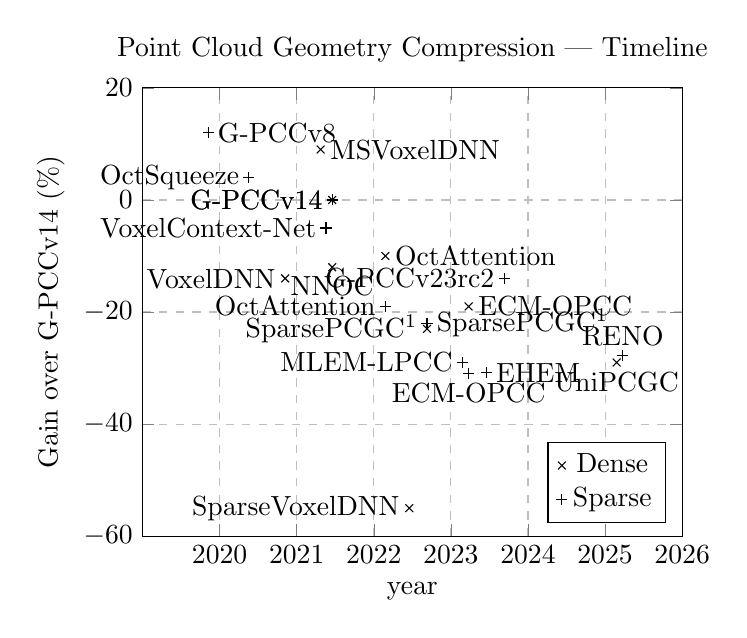
\begin{tikzpicture}
\begin{axis}[
    title={Point Cloud Geometry Compression --- Timeline},
    xlabel={year},
    ylabel={Gain over G-PCCv14 (\%)},
    xmin=2019, xmax=2026,
    ymin=-60, ymax=20,
    xtick={2020, 2021, 2022, 2023, 2024, 2025, 2026},
    ytick={-60, -40, -20, 0, 20},
    legend pos=south east,
    xmajorgrids=true,
    ymajorgrids=true,
    grid style=dashed,
    /pgf/number format/.cd,
    set decimal separator={.},
    1000 sep={},
    fixed,
]

\addplot[
    color=black,
    mark=x,
    only marks,
    point meta = explicit symbolic,
    nodes near coords,
    visualization depends on=\thisrow{align} \as \align,
    every node near coord/.style={anchor=\align}
]
table[meta=label] {
    x       y   label           align
    2020.85 -14  VoxelDNN        0
    2021.46 -12  NNOC            90
    2021.31 9    MSVoxelDNN      180
    2021.46 0    G-PCCv14        0
    2022.69 -23  SparsePCGC$^1$  0
    2022.15 -10  OctAttention    180
    2022.46 -55  SparseVoxelDNN  0
    2023.23 -19  ECM-OPCC        180
    2025.15 -29  UniPCGC         90
};
\addlegendentry{Dense}

\addplot[
    color=black,
    mark=+,
    only marks,
    point meta = explicit symbolic,
    nodes near coords,
    visualization depends on=\thisrow{align} \as \align,
    every node near coord/.style={anchor=\align}
]
table[meta=label] {
    x       y     label             align
    2019.85 12    G-PCCv8           180
    2020.38 4     OctSqueeze        0
    2021.38 -5    VoxelContext-Net  0
    2021.46 0     G-PCCv14          0
    2022.69 -22   SparsePCGC$^1$    180
    2022.15 -19   OctAttention      0
    2023.15 -29   MLEM-LPCC         0
    2023.23 -31   ECM-OPCC          90
    2023.46 -30.8 EHEM              180
    2023.69 -14   G-PCCv23rc2       0
    2025.23 -27.8 RENO              270
};
\addlegendentry{Sparse}

%MDPI: 1. Commas are only used for numbers with five or more digits. Please remove them from the four-digit numbers in the figure, e.g., “1,200” should be “1200”. 2. Please add an explanation of *.
%AUTHORS: Found config to remove unwanted commas.
%AUTHORS: That * next to G-PCCv14 is no asteriks but the overlap of +/x, readers will notice, AI probably not.
%AUTHORS: We tried to replace $^1$ with \dagger, but it looks more confusing. We stick to $^1$.
%AUTHROS: Explanation was always there!
\end{axis}
\end{tikzpicture}
\caption{The timeline of key publications in lossless point cloud geometric compression over the past half decade,
illustrating the steady performance improvements achieved relative to the G-PCCv14 baseline.
$^1$SparsePCGC was originally published in November 2021 with comparatively lower performance due to hardware limitations at the time.
With the advent of newer GPUs such as the NVIDIA RTX 4090, larger model configurations and reduced inference times have become feasible, resulting in significantly improved compression performance.
\label{fig:timeline}}
\end{figure}

%MDPI: We've removed the vertical lines of all tables, please confirm.
%AUTHORS: Thank your. We wish to keep the vertical lines for better readiness.
%AUTHORS: \cmidrule looks terrible - don't use that, please.
\begin{table}[H]
\caption{
\label{tab:related_works}%
A set of deep learning-based entropy models for geometric point cloud compression,
grouped and categorized by their input features, primary context modeling components,
output probability representations, and autoregressive level.
The last two columns on the right summarize the relative compression performance gain$^{-1}$ over G-PCCv14 and the decoding time for both sparse and dense point clouds.
}
%\centering
\tabcolsep=0.185cm
%\begin{adjustwidth}{-\extralength}{0cm}
{
\renewcommand{\baselinestretch}{1}\small
\isPreprints{\centering}{}
\begin{tabularx}{\textwidth}{c|c|c|c|c|c|c}
%\begin{tabular}{c|c|c|c|c|c|c}

%MDPI: Please check if `..' should be changed to a single decial point or $\ldots$. Same as below.
%AUTHORS: Thank you. Dots have been replaced
\toprule
\thead{Name} & \thead{Input} & \thead{Context Model} & \thead{Output} & \thead{Auto-\\Regressive} & \thead{Sparse\\Dense} & \thead{Time} \\
\midrule
MIC-OPCCv2 & \makecell{location,\\occupancy\\(binarized)} & \makecell{Index\\Convolution} & \multirowcell{12}{voxels\\0\dots1} & \multirowcell{3}{semi} & \makecell{32.6\%\\30.6\%} & \makecell{3.5 s\\5 s} \\
\cline{1-3}\cline{6-7}
MSVoxelDNN & \multirowcell{13}{voxels} & \multirowcell{6}{Masked\\3D-Convolution} & & & \makecell{-\\$-$9.7\%} & \makecell{-\\58 s} \\
\cline{5-7}
VoxelDNN & & & & \multirowcell{6}{fully} & \makecell{-\\13.9\%} & \makecell{-\\640 s} \\
\cline{6-7}
NNOC & & & & & \makecell{-\\11.5\%} & \makecell{-\\1171 s} \\
\cline{3-3}\cline{6-7}
SparseVoxelDNN & & \makecell{Masked \& Sparse\\3D-Convolution} & & & \makecell{-\\52.8\%} & \makecell{-\\229 s} \\
\cline{3-3}\cline{5-7}
SparsePCGC & & \multirowcell{6}{Sparse\\3D-Convolution} & & \multirowcell{3.5}{semi} & \makecell{22.0\%\\33.8\%} & \makecell{1.2 s\\1.9 s} \\
\cline{6-7}
UniPCGC & & & & & \makecell{-\\29.2\%} & \makecell{-\\0.57 s} \\
\cline{1-2}\cline{4-7}
RENO & \makecell{occupancy\\(embedded)} & & & & \makecell{17.8\%\\-} & \makecell{0.1 s\\-} \\
\cline{1-2}\cline{3-3}\cline{6-7}
Voxel-Context Net & voxels & 3D-Convolution & \multirowcell{14}{\\octree\\nodes\\1\dots255} & \multirowcell{7}{none} & \makecell{8.1\%\\-} & \makecell{0.09 s\\-} \\
\cline{1-3}\cline{6-7}
MIC-OPCCv1 & \makecell{location,\\occupancy\\(binarized)} & \makecell{Index\\Convolution} & & & \makecell{19.6\%\\30.6\%} & \makecell{2.5 s\\5.0 s} \\
\cline{1-3}\cline{6-7}
OctSqueeze & \makecell{location,\\occupancy,\\level,\\octant} & \makecell{Multi-Layer\\Perceptron\\(MLP)} & & & \makecell{$-$2.1\%\\-} & \makecell{0.08 s\\-} \\
\cline{1-3}\cline{5-7}
OctAttention & \multirowcell{6}{occupancy,\\level,\\octant\\(embedded)} & \multirowcell{6}{breadth-first\\transformer} & & fully & \makecell{19.5\%\\9.7\%} & \makecell{530 s\\1229 s} \\
\cline{5-7}
ECM-OPCC & & & & \multirowcell{3}{semi} & \makecell{32.6\%\\19.5\%} & \makecell{-\\19.8 s} \\
\cline{6-7}
EHEM & & & & & \makecell{32.6\%\\-} & \makecell{0.43 s\\-} \\
\bottomrule

\end{tabularx}
}
%\end{adjustwidth}
\end{table}

\subsection{Voxel-Based Entropy Models}
These methods employ 3D convolutions over voxelized occupancy grids.
However, due to the cubic complexity $O(n^3)$, high-resolution voxelization can quickly exceed hardware capacity.
Nguyen~{et al.} introduced VoxelDNN~\citep{VoxelDNN}, inspired by PixelCNN~\citep{PixelCNN}, which partitions point clouds into $64^3$ voxel blocks and uses masked 3D convolutions in a fully autoregressive manner to predict voxel occupancy probabilities.
Kaya~{et al.} proposed \acrshort{NNOC}~\citep{NNOC}, which explores the voxel grid layer by layer, but both models remain fully autoregressive and hence computationally expensive.
MSVoxelDNN~\citep{MSVoxelDNN} partially relaxes the autoregressive dependency, achieving parallelism at the cost of higher bitrates.

Sparse convolution frameworks such as the Minkowski Engine~\citep{Minkowski,SparseCNN} allow high-resolution processing.
This enabled Wang~{et al.} to develop SparsePCGC~\citep{SparsePCGC}, capable of 12-bit precision using sparse convolution with an 8-stage autoregressive model.
Later, \acrshort{UniPCGC}~\citep{UniPCGC} proposed a refined grouping strategy, arguing that early-stage voxels provide underrepresented spatial information.
By skipping select voxels in initial groups and expanding later stages, \acrshort{UniPCGC} improved both compression ratio and decoding time compared to SparsePCGC.
SparseVoxelDNN~\citep{SparseVoxelDNN} is namely the transition of VoxelDNN~\citep{VoxelDNN} from dense convolution to sparse convolution.

\subsection{Octree-Based Entropy Models}
Octree-based approaches decompose point clouds hierarchically, enabling localized feature extraction per node.
OctSqueeze~\citep{OctSqueeze} was the first end-to-end octree-based model, predicting the 8-bit occupancy symbol of each node using a \acrfull{MLP} that processes ancestor features.
However, its lack of neighborhood search and autoregression limited effectiveness, and later voxel-based approaches surpassed it.
Recent octree models, including OctAttention~\citep{OctAttention}, \acrshort{ECM-OPCC}~\citep{ECM-OPCC}, and \acrshort{EHEM}~\citep{EHEM}, leverage attention mechanisms such as transformers to capture hierarchical dependencies.
They convert octrees into deterministic sequences (e.g., breadth-first order), allowing transformers to model autoregressive dependencies efficiently.
Yet, the breadth-first ordering only approximates neighborhood relations and does not always reflect true spatial proximity.
While these transformer-based methods excel in sparse point clouds, they are computationally heavy.
For example, ECM-OPCC~\citep{ECM-OPCC} achieves strong compression performance but requires 19.5~s for decoding and nearly exhausts 40~GB of GPU memory, limiting real-time applicability.
EHEM~\citep{EHEM} introduces a \textit{{hierarchical attention mechanism}} designed to accelerate decoding by efficiently expanding the receptive field.
It first merges the features of sibling nodes before applying the transformer, and then up-samples them back to their original resolution.
This hierarchical fusion strategy effectively broadens the spatial context at low computational cost, demonstrating particular efficiency for sparse point clouds.

\subsection{Hybrid Entropy Models}
Hybrid models combine multiple representations---such as octrees, voxelization, and spatial coordinates---offering a balance between granularity and efficiency.
VoxelContextNet~\citep{VoxelContextNet} encodes octrees but converts each node into small voxel blocks $(11^3)$ for 3D convolutional feature extraction.
The more recent \acrshort{RENO}~\citep{RENO} uses sparse convolution with embedded occupancy features (32 channels per voxel) and two autoregressive stages.
Our proposed MIC-OPCCv2 consumes point-based features while maintaining an octree structure, but encodes each occupancy symbol bit-by-bit in a voxel-wise manner.

\subsection{Summary}
In summary, Table~\ref{tab:related_works} provides a structured comparison of leading deep learning-based \acrshort{pcgc} methods.
We categorize these models according to four key aspects:

\begin{enumerate}
    \item Type of input features;
    \item Main context modeling component;
    \item Type of probability output;
    \item Level of autoregression.
\end{enumerate}

%MDPI: We move it to here, please check
The final two columns report their compression performance on sparse versus dense point clouds and their decoding times.
All results are cited faithfully from original sources.
It is evident that fully autoregressive models achieve strong compression but at impractical decoding times.
Semi-autoregressive methods address this limitation through architectural enhancements or model scaling.
Finally, voxel-based approaches tend to perform better on dense point clouds, whereas octree-based methods excel on sparse data.

Projection-based methods are excluded from this survey due to their inherent limitations.
For instance, \acrshort{RIDDLE}~\citep{RIDDLE} applies only to single range image frames from individual sensors, whereas many real-world point clouds are composites from multiple scans and sensors~\citep{8iVFBv2,MVUB,Waymo,NuScene}.

Despite significant progress, existing methods continue to face key trade-offs between compression efficiency, decoding speed, and memory consumption.
Fully autoregressive models achieve superior bitrates but suffer from prohibitively long decoding times, while semi-autoregressive or sparse convolution methods often sacrifice accuracy for faster inference.
Transformer-based octree models, though highly expressive, require extensive computational resources and large memory footprints, making them unsuitable for real-time applications or deployment on embedded systems.
To address these challenges, we propose MIC-OPCCv2, a lightweight and computationally efficient hybrid entropy model based on multi-index 1D convolution.
Our approach captures spatial context through dynamically ordered convolutions, achieving fast decoding with competitive compression performance---bridging the gap between traditional octree-based and voxel-based neural~codecs.

\section{Background}
\label{sec:background}

Our method builds on the same foundational principles as previous works, leveraging Shannon's theorem~\citep{Shannon}, which defines the entropy $h$ of a symbol $s$ as
\begin{equation}
h(s) = -\log_2{p(s)}.
\label{equ:shannon}
\end{equation}

This formulation defines the entropy $h$ as the theoretically required number of bits to represent a symbol $s$, where the probability $p(s)$ lies within the range $0 < p(s) < 1$.
During decoding, however, the true probability distribution $p(s)$ is uncertain and can only be approximated by a stochastic, heuristic, or empirical model. We express this approximation~as
\begin{equation}
q(\mathbf{x}) = \mathbf{\hat{y}},
\label{equ:uncertainty}
\end{equation}
where $\mathbf{y}$ is a one-hot encoded vector representing the ground truth symbol $s$, and $\mathbf{\hat{y}}$ is the estimated probability distribution inferred from the contextual input $\mathbf{x}$.
Our goal is to optimize $q_\theta(\mathbf{x})$---a parameterized empirical model, such as one driven by deep learning---by minimizing the cross-entropy between $\mathbf{y}$ and $Q_\theta(x_i)$:

\begin{equation}
H(y, x) = -\sum_{i=1}^{n} y_i \log{Q_\theta(x_i)},
\label{equ:crossentrop}
\end{equation}
where $H(y, x)$ measures the divergence between the true and estimated distributions.
An Arithmetic Encoder~\citep{Arithmetic} can then transform the symbol $s$ into a compact bitstream, with the efficiency of the encoding directly tied to the accuracy of the probability estimate $Q_\theta(x_i) = \mathbf{\hat{y}}_i$.

\subsection{Binary Arithmetic Coding}
\label{sec:bac}
Arithmetic coding is a form of entropy encoding used in lossless data compression.
Unlike Huffman coding~\citep{Huffman}, which assigns discrete bit patterns to each symbol, arithmetic coding encodes an entire message into a single fractional number within the interval $[0, 1)$.
This approach allows for fractional bit efficiency, resulting in compression rates close to the theoretical entropy limit.

In arithmetic coding, a message is represented by a progressively refined numerical interval.
Each new symbol subdivides the current interval into smaller partitions according to its estimated probability.
The more probable a symbol is, the smaller the range reduction it induces---thus requiring fewer bits to encode.
This recursive subdivision continues for all symbols in the message, producing an increasingly precise numerical representation.
When the final interval is specified to sufficient precision, its binary representation serves as the compressed output.

\acrfull{bac}, a simplified form of arithmetic coding, performs recursive interval subdivision based on binary decisions between the most probable symbol and the least probable symbol.
The interval width corresponds to the product of the symbol probabilities, and the binary representation of the final interval asymptotically approaches the Shannon theorem's lower bound on entropy.
A key advantage of BAC is its clean separation between modeling and coding, allowing a probability model to be optimized independently from the coding engine---a property central to our proposed approach.

\subsection{Fast Octree Coder}
\label{sec:octree}

An octree provides an efficient means of organizing unstructured and unsorted data through recursive spatial partitioning~\citep{Octree}.
However, costly spatial computation and floating-point arithmetic can be avoided by \acrfull{foc} as shown in Figure~\ref{fig:octree}.
\acrshort{foc} simply groups a pre-quantized point cloud $Q$ based on the $t$ most significant bits of each component in a quantized point $\mathbf{q}=\mathbf{p}_{b_{L-t}}$, where $t$ reflects the current quantization level and tree depth.
Each group raises a bit on the 8-bit occupancy symbol $s$ according to its octant signature at position $t$.
This algorithm allows fast random access to any depth-level in the tree at a complexity of $\mathcal{O}(\log_{2}n)$

\begin{figure}[H]
%\centering
%MDPI: Please confirm whether the dashed box and dashed line need explanation.
\includegraphics[width=1.0\textwidth]{mic-opcc/figures/Octree.pdf}
\caption{Fast Octree Coding. Any octree level at depth $t$ can be constructed instantly with a complexity of $\mathcal{O}(\log_{8} n)$ by grouping points according to their $3t$ most significant bits, enabling efficient hierarchical partitioning of the quantized point cloud.}
\label{fig:octree}
\end{figure}

A breadth-first traversal of the octree, expressed as $S = \{\mathbf{s}_0 = (s_0, \dots, s_j), \dots, \mathbf{s}_L\}$, typically yields much lower entropy per symbol $s$ than the raw spatial coordinates $\mathbf{p} = (x, y, z)$ of a point cloud $P$.

Earlier octree-based models, such as OctSqueeze~\citep{OctSqueeze}, included the real-valued positions of each octree-node as features.
However, the absence of real position values in recent works~\citep{OctAttention,ECM-OPCC,EHEM,UniPCGC,RENO} implies that this feature is less effective for spatial context modeling.
Instead, embedded occupancy flags, 3-bit octants, and quantization depth provide more discriminative and compact features.

\section{Methodology}
\label{sec:methods}

Building upon the limitations identified in prior research, we propose MIC-OPCCv2---an enhanced version of our lightweight multi-index convolutional entropy model~\citep{MIC-OPCCv1} designed for efficient octree-based point cloud compression.
An overview of the framework is provided in Figure~\ref{fig:model_overview}. The architecture integrates four key components:
\begin{enumerate}
    \item A \textit{{progressive grouping}} scheme, which introduces autoregressive dependencies between voxel candidates at identical resolution levels;
    \item A \textit{{blender \& distiller}} network, which refines hierarchical representations through residual feature aggregation;
    \item A \textit{{multi-index convolution}} backbone, enabling spatially coherent context extraction at minimal computational cost;
    \item \textls[-25]{A \textit{{binary location}} encoder, serving as a compact and expressive geometric feature~representation.}
\end{enumerate}

\begin{figure}[H]
%\centering
%MDPI: Please confirm whether the dashed boxes, boxes with different lines,  yellow/blue squares and solid/dashed arrows require explanation.
%AUTHORS: This is an overview, details descriptions are in methods
\includegraphics[width=1.0\textwidth]{mic-opcc/figures/ModelOverview.pdf}
\caption{
Overview of the MIC-OPCCv2 architecture.
The input point cloud is quantized and binarized to form an octree representation.
Each octree-node expands into eight voxel candidates, which are arranged into eight autoregressive groups following the progressive grouping scheme.
Each group is processed by the blender \& distiller network using multi-index convolution to estimate occupancy probabilities.
These probabilities are consumed by a \acrshort{bac} during compression and are supervised through categorical cross-entropy during training.
The resulting occupancy symbols can be converted back into an octree and subsequently into a reconstructed quantized point cloud.
Arrows indicate data flow, unless further descriped.
All core modules are further descriped in Section~\ref{sec:methods}.
}
\label{fig:model_overview}
\end{figure}

%MDPI:We move it to here, please check
Together, these components allow MIC-OPCCv2 to achieve competitive or state-of-the-art compression performance while operating with significantly lower memory usage and substantially reduced decoding complexity compared to existing neural \acrshort{pcgc} methods.

The following sections detail the core elements of the proposed codec. Section~\ref{sec:index_convolution} introduces the multi-index convolution mechanism. Sections~\ref{sec:blender_and_distiller} and \ref{sec:progressive_grouping} describes the blender \& distiller network and the progressive grouping strategy. Section~\ref{sec:binary_locations} outlines the construction of binarized location features, and Section~\ref{sec:loss_function} presents the training objective and loss formulation.

\subsection{Index Convolution}
\label{sec:index_convolution}

Transformer-based methods~\citep{OctAttention,ECM-OPCC,EHEM} process octree-nodes sequentially following a breadth-first traversal order.
However, this neighborhood ordering is not always spatially consistent, as nearby points or voxels may appear far apart in the traversal sequence as octree-nodes.
To overcome this limitation, we introduce a multi-index 1D convolution~operation, illustrated in Figure~\ref{fig:index_convolution}.

For each spatial dimension, an \texttt{arg-sort} operation generates an index that defines the processing order.
This index is created once at the beginning.
The point features are then reordered according to this index before applying 1D convolution.
After convolution, the outputs are reverted to their original order using the inverse index and aggregated.
Repeating this process across all dimensions progressively enlarges the model's receptive field, enabling the aggregation of broader spatial dependencies.

\begin{figure}[H]
%\centering
%MDPI: 1. Please cite this figure in the text and ensure that the first citation of each figure appears in numerical order. 2. Please confirm whether an explanation of the Pink/orange/purple squares and arrows needs to be added to the figure caption. 3. The figure should be placed below its first-mentioned paragraph and must not cross section headings. However, to minimize white space, please assess if it can be moved to follow the Heading 4.1 paragraph after the citation is inserted there, and confirm if this is acceptable.
%AUTHORS: Figure is now cited
%AUTHORS: More explination of the obvious
\subfloat[\centering]{\includegraphics[width=0.44\textwidth]{mic-opcc/figures/IndexConvolution_a.pdf}}\hspace{-6pt}
\hfill
\subfloat[\centering]{\includegraphics[width=0.55\textwidth]{mic-opcc/figures/IndexConvolution_b.pdf}}
\caption{
Illustration of the proposed multi-index 1D convolution framework,
which reorders spatial features along multiple dimensions to form directionally variant receptive fields.
Each convolution output is reverted and aggregated in the original order to accumulate contextual information in all~directions.
(\textbf{a}) presents a visual example of the multi-index convolution using four different orderings $(x,y,z,q)$, highlighted in distinct colors and combined by summation.
(\textbf{b}) provides a schematic overview of the processing pipeline, with arrows indicating the data flow.
}

\label{fig:index_convolution}
\end{figure}

Our indexed convolution can be interpreted as an approximated low-complex $k$-nearest-neighbor lookup along fixed axes, effectively merging adjacent voxels in sorted order.
Unlike previous methods that rely on zero-padding for empty voxels within a fixed receptive window, our approach ensures that only existing voxels contribute to the receptive field.
This dynamic adaptation allows the model to handle sparse regions more effectively by implicitly adjusting the receptive field size.

\subsection{Blender \& Distiller}
\label{sec:blender_and_distiller}

Samples in \acrshort{pcgc} exhibit a wide range of entropy characteristics.
Low-resolution samples tend to emit low entropy, while high-resolution samples approach near-random distributions with substantially higher entropy.
Consequently, prior research has emphasized the value of residual network architectures to accommodate such variability~\citep{ResNet,UniPCGC,SparseVoxelDNN}.
The underlying intuition is that low-entropy samples can be effectively modeled with shallow networks, whereas high-entropy samples require deeper networks capable of capturing more complex causal dependencies.

Voxel occupancy estimation, as formulated in \acrshort{pcgc}, is conceptually analogous to image segmentation.
In this domain, U-Net architectures~\citep{UNet,MultiResUNet} have demonstrated superior performance compared to conventional ResNet-based models, primarily due to their ability to combine multi-scale contextual information through skip connections.
Inspired by these findings, we propose a blender \& distiller architecture, illustrated in Figure~\ref{fig:blender_and_distiller}.

In our design, the blender layers act as recursive feature aggregators that combine information across different receptive fields.
Aggregation can be achieved through summation, concatenation, convolution, or attention-based fusion.
In our case, multi-index convolution serves as the primary aggregation mechanism, progressively refining spatial context representations across hierarchical depth.
Each blender layer thus produces increasingly complex hidden features, with deeper layers contributing to broader spatial understanding.
\begin{figure}[H]
%\centering
%MDPI: Please confirm whether an explanation of the arrow needs to be added to the figure caption.
%AUTHORS: Thank you. Explanation is added.
\hspace{-12pt}\includegraphics[width=1.0\textwidth]{mic-opcc/figures/BlenderAndDistiller.pdf}
\caption{
The proposed \textit{{blender \& distiller}} architecture is a strongly residual framework inspired by U-Net~\citep{UNet},
but differs by incorporating a multi-stage voting mechanism on the output side, where each distiller contributes to the final probability estimation.
The left panel presents an abstract schematic of the architecture, while the right panel illustrates a concrete implementation example.
Dashed boxes denote placeholders for repeated layers, and arrows indicate the direction of data flow.
}
\label{fig:blender_and_distiller}
\end{figure}
The distiller layers, on the other hand, are responsible for extracting probability estimations from each blender stage.
Their outputs are subsequently combined through a normalized summation, effectively forming a collective ``vote'' across all hierarchical levels of the network.
This mechanism enforces contribution from every stage, ensuring that intermediate representations meaningfully participate in the final prediction.
Empirically, this voting-based mechanism proves highly effective for \acrshort{pcgc}, as it maintains strong contextual awareness across both local and global spatial scales.

Unlike the U-Net~\citep{UNet}, our design omits connections between distiller inputs, simplifying the data flow while maintaining hierarchical feature consistency.
For binary classification tasks, each distiller outputs two positive unconstrained logits.
This formulation allows a distiller to either abstain from contributing (by emitting near-zero magnitudes) or to dominate the final consensus when confident.
Through backpropagation, each distiller dynamically adjusts its contribution to the aggregate prediction, facilitating adaptive behavior across samples of varying entropy.

Formally, the aggregated output of all $N$ distillers is expressed as
\begin{gather}
F^{N+1}_{t,g} = \sum_{i=1}^{N}{\text{Distiller}_i(F^i_{t,g})}, \\
Q_\theta\left(C_{t,g} \middle| O_{<(t,g)}\right) = \text{SoftMax}(F^{N+1}_{t,g}),
\label{eq:distiller_sum}
\end{gather}
where $\text{Distiller}_i(F^i_{t,g})$ denotes the $i$-th distiller output operating on hidden features $F^i_{t,g}$ derived from the preceding blender layer.
The softmax normalization converts the summed logits into a probability distribution $Q_\theta(C_{t,g} | O_{<(t,g)})$, which represents the estimated occupancy likelihood for voxel candidates $C_{t,g}$ conditioned on the previously decoded occupancies $O_{<(t,g)}$.

These probabilities directly feed into the categorical cross-entropy loss described in Section~\ref{sec:loss_function}, ensuring that learning is guided by the aggregated multi-scale consensus of all distillers.
In this way, the \emph{blender \& distiller} network forms a mathematically consistent bridge between spatial feature extraction and probabilistic entropy modeling, enabling efficient and robust learning across diverse octree resolutions.

\begin{figure}[H]
%\centering
%MDPI: 1. Please cite this figure in the text and ensure that the first citation of each figure appears in numerical order. 2. Please confirm if “[number]” in the figure are reference citations. If so, references in the form [XX] are not permitted in images. Please move the reference to the figure caption. If necessary, please use the format of “Author+Year” in the image instead, and all references mentioned should be cited in the caption.
%AUTHORS: No these are no citations, we changed the style to prevent confusion.
\includegraphics[width=0.75\textwidth]{mic-opcc/figures/AutoRegressiveGrouping.pdf}
\caption{Progressive grouping strategy of MIC-OPCCv2.
Each octree-node $\mathbf{o}_i$ expands into a block of eight voxel candidates $v$.
For every autoregressive group, voxel candidates are selected according to a stride $s$, an offset $o$, and a target index $v$.
Early groups operate under limited spatial context and therefore decode only a subset of voxels, enabling more reliable probability estimation for later groups.
As contextual information accumulates, later groups increase throughput by decoding multiple voxels concurrently.}
\label{fig:progressive_grouping}
\end{figure}

\subsection{Progressive Grouping}
\label{sec:progressive_grouping}

To incorporate autoregressive dependencies while avoiding the high latency of fully sequential decoding, we adopt a grouped decoding strategy inspired by UniPCGC~\citep{UniPCGC}, which itself extends the SparsePCGC~\citep{SparsePCGC} framework.
Rather than decoding voxels strictly one-by-one, grouping strategies partition voxel candidates into subsets that are decoded iteratively, enabling a controlled trade-off between contextual refinement and parallelism.
We collectively refer to these approaches as variants of autoregressive grouping strategies.

In this work, we implement a progressive grouping strategy, illustrated in Figure~\ref{fig:progressive_grouping}, that dynamically adjusts the grouping granularity across decoding stages.
The key motivation is that early decoding decisions are made under limited contextual information and therefore benefit most from fine-grained autoregressive conditioning, whereas later decisions can be decoded more aggressively once the occupancy distribution becomes increasingly constrained.
Accordingly, the first decoding stages process a reduced candidate set by activating only every second voxel, which limits parallelism but maximizes contextual reliability.
As decoding progresses, the grouping size is gradually increased, allowing more voxel candidates to be decoded per iteration while leveraging the richer context accumulated from earlier stages.

This progressive schedule differs from sequential grouping or fully autoregressive methods in that it explicitly adapts the balance between context accuracy and decoding throughput over time.
It also avoids excessive sequential dependency chains, which would otherwise dominate decoding latency.
Empirically, we observe that this ordering provides a favorable compromise between compression efficiency and runtime compared to alternative grouping strategies, such as sequential grouping~\citep{SparsePCGC} or fully voxel-wise autoregression~\cite{SparseVoxelDNN}.
Nevertheless, we note that the effectiveness of progressive grouping depends on the spatial distribution of occupied voxels: for highly dense or highly regular structures, overly aggressive grouping in later stages may reduce contextual precision.

Overall, the proposed progressive grouping strategy enables efficient autoregressive modeling with linear-time decoding complexity, while preserving most of the rate-distortion benefits of fine-grained context modeling.

\begin{figure}[H]
%\centering
%MDPI: 1. Please cite this figure in the text and ensure that the first citation of each figure appears in numerical order. 2. Please change the hyphen (-) into a minus sign (−, “U+2212”) in the figure, e.g., “-1” should be “−1”.
%MDPI: Please confirm whether an explanation of the background color needs to be added to the figure caption.
%AUTHORS: Thank you, figure is now cited
%AUTHORS: Thank you, fixed the character (−, “U+2212”)
%AUTHORS: Thank you, added a legend
\includegraphics[width=0.75\textwidth]{mic-opcc/figures/Feature-Generator.pdf}
\caption{Illustration of the binarization, normalization, and masking process for feature generation at quantization level $L=8$ and current coding depth $t=5$. Bits beyond the current depth are masked to prevent access to unavailable information during decoding.}
\label{fig:binary_locations}
\end{figure}

\subsection{Binary Location Encoding}
\label{sec:binary_locations}

The preprocessing pipeline used for our model input is illustrated in Figure~\ref{fig:binary_locations}.
Each point $\mathbf{p} = (x, y, z) \in \mathbb{R}$ is first normalized and quantized according to
\begin{gather}
\mathbf{q} = \left\lfloor \frac{2^L}{s}(\mathbf{p} - o) \right\rfloor,
\end{gather}
ensuring all coordinates are positive and confined to the range $[0, 2^L)$.
A binarization function generates bit-level representations:
\begin{gather}
b_i(p) = \left\lfloor \frac{p}{2^i} \right\rfloor \bmod 2,
\end{gather}
and concatenation across axes produces hierarchical binary descriptors:
\begin{gather}
\mathbf{b}_L(\mathbf{q}) = [b_{L-1}(z), b_{L-1}(y), b_{L-1}(x), \dots, b_0(z), b_0(y), b_0(x)].
\end{gather}

%MDPI: Please confirm if indentation is required and check the whole text.
%AUTHORS: Thank you, probably not.
A mask $\mathbf{m}_{td}$ ensures that only information up to the current decoding depth $t$ is visible:
\begin{gather}
m_i =
\begin{cases}
1, & \text{if } i < td, \\
0, & \text{otherwise}
\end{cases}.
\end{gather}

Finally, the masked binary features are centered to $[-0.5, 0.5]$ to distinguish true zeros from masked bits:
\begin{gather}
F^0 = \left\{ \left( \mathbf{b}_L(\mathbf{p}_j) - 0.5 \right)\mathbf{m}_{td} \mid \forall j \right\}.
\end{gather}

Using this binarization scheme, variant indices $I$ can be derived for different voxel orderings, enabling diverse spatial perspectives in the multi-index convolution process.
By summing the bits across the quantization levels $L$ and dimensions $d$, we obtain an index $I_q$ corresponding to the breadth-first traversal order of an octree:\vspace{-3pt}
\begin{gather}
I_q = \left\{ \sum^{L-1}_{k=0}\sum^3_{d=1}{b_{t}(p_d)2^{3t+d-1}} \middle| \forall \mathbf{p}=(x,y,z) \right\}.
\end{gather}

Alternatively, by summing the binary bits along dimensions first and then over quantization levels, we derive axial voxel orderings, such as $I_{x}$, $I_{y}$, and $I_{z}$:
\begin{gather}
I_{x} = \left\{ \sum^3_{d=1}\sum^L_{t=1}{b_{L-t}(p_d)2^{Ld-t}} \middle| \forall \mathbf{p}=(x,y,z) \right\}, \\
I_{y} = \left\{ \sum^3_{d=1}\sum^L_{t=1}{b_{L-t}(p_d)2^{Ld-t}} \middle| \forall \mathbf{p}=(y,z,x) \right\}, \\
I_{z} = \left\{ \sum^3_{d=1}\sum^L_{t=1}{b_{L-t}(p_d)2^{Ld-t}} \middle| \forall \mathbf{p}=(z,x,y) \right\}.
\end{gather}

By cyclically swapping the dimensional components in $\mathbf{p}$, we obtain different axial orderings for each dimension $d$.
These variant indices serve as sorting references for our multi-index convolutions, allowing the model to perceive spatial relationships from multiple directional perspectives.

\subsection{Loss Function}
\label{sec:loss_function}

The training objective of MIC-OPCCv2 is to minimize the categorical cross-entropy loss between the predicted probability distribution $P_{t,g}$ and the true occupancy label $O_{t,g}$ for each voxel, across all resolution levels $t$, and autoregressive groups $g$. The loss function is formulated as
\begin{gather}
\mathcal{L}_{t,g} = \mathbb{E}_{O_{t,g} \sim P_{t,g}}\left[-\log \mathcal{Q}_\theta(C_{t,g} \middle| O_{<(t,g)})\right],
\label{eq:loss}
\end{gather}
where $\mathcal{Q}_\theta$ represents our probability estimation model parameterized by $\theta$, applied over the current voxel candidates $C_{t,g}$ and the already processed occupancy symbols $O_{<(t,g)}$ from previous decoding steps.

For each target voxel, the model outputs two class probabilities---occupied versus empty---using a softmax activation applied to the final feature representation $F^{N+1}_{t,g}$, as defined in Equation~\eqref{eq:distiller_sum}.

Each distiller layer $\text{Distiller}_i$ implements a fully connected (dense) layer with kernel size $k=2$, using \textit{SoftPlus} for unbound positive activation:
\begin{gather}
\text{Distiller}_i(F^i_{t,g}) = \text{SoftPlus}\left(\text{Dense}_i^{k=2}(F^i_{t,g})\right).
\label{eq:distiller}
\end{gather}

The input features $F^i_{t,g}$ correspond to the subset of encoded voxels $T_{t,g}$ at the current stage $i$, defined as
\begin{gather}
F^i_{t,g} = \{ x \mid \forall n \in T_{t,g} : x_n \in F^i \}.
\end{gather}

The distillers extract two scalar outputs per voxel, corresponding to the probability logits of occupancy and emptiness. These logits are derived from the recursively accumulated hidden features $F^i$, obtained via the \textit{blender layers}:\vspace{-3pt}
\begin{gather}
F^i = \text{Blender}_i(F^{i-1}),
\end{gather}
where each blender performs feature aggregation across all spatial indices using layer normalization and ReLU activation:\vspace{-3pt}
\begin{gather}
\text{Blender}_i(F^{i-1}) = \text{LayerNorm}\left(
\sum_{d=1}^{4}
\text{ReLU}\left(
\text{IndexConv}^{k=64}_{i,d}(F^{i-1}, I_d)
\right)
\right).
\label{eq:blender}
\end{gather}

This formulation summarizes four index convolutions with different sorting orders $I_d$, starting from the initial feature set $F^0$:
\begin{gather}
F^0 = \left\{ \mathbf{b}_L(\mathbf{p}) \mid
\forall \mathbf{p} \in \bigcup \{ C_{t,g}, O_{<(t,g)} \} \right\},
\label{eq:f0}
\end{gather}
where $\mathbf{b}_L(\mathbf{p})$ represents the binarized and serialized feature vector of spatial locations $\mathbf{p}$.
Here, $O_{<(t,g)}$ refers to all decoded voxels from prior steps, and $C_{t,g}$ represents candidate voxels generated for the current group.
Our overall probability mass function is therefore
\begin{gather}
\mathcal{P}_\theta(\mathcal{O}) = \prod_{t=1}^{L}\prod_{g=1}^{G=8}\mathcal{Q}_\theta\left(C_{t,g} \middle| O_{<(t,g)}\right).
\label{eq:mass}
\end{gather}

This autoregressive structure allows MIC-OPCCv2 to iteratively refine spatial and contextual representations across layers and groups, improving the accuracy of occupancy probability estimation for each voxel candidate.

\subsection{Model Splitting}
\label{sec:model_splitting}

Each octree level exhibits distinct entropy characteristics due to the hierarchical refinement of spatial resolution, as illustrated in Figure~\ref{fig:variance_plot}.
The upper levels near the root generally show low entropy, since most nodes are fully occupied when the point cloud is centered.
Intermediate levels contain the widest variety of occupancy patterns and therefore present the highest entropy.
At deeper levels, although spatial precision increases, occupancy becomes sparse and the entropy decreases again, as fully occupied patterns are rare.


\vspace{-12pt}

\begin{figure}[H]
\pgfplotsset{
    width=\textwidth*0.45,
    tick label style={font=\footnotesize},
    label style={font=\small},
    legend style={font=\tiny},
}
%\isPreprints{}{% This command is only used for ``preprints''.
%\begin{adjustwidth}{-\extralength}{0cm}
\centering
%} % If the paper is ``preprints'', please uncomment this parenthesis.

%\begin{adjustwidth}{-\extralength}{0cm}
%\centering %% If there is a figure in wide page, please release command \centering, for Table, ``\textwidth" should be ``\fulllength"
\subfloat[\centering]{
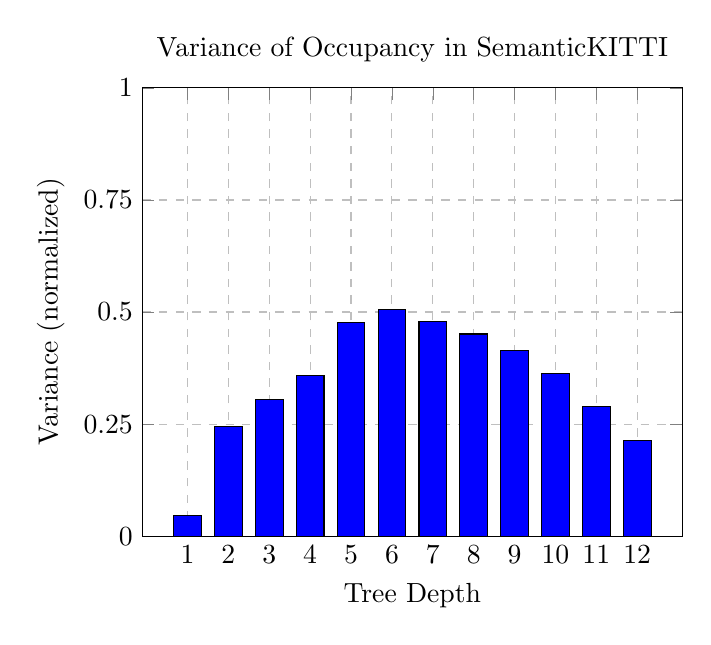
\begin{tikzpicture}
\begin{axis}[
    title={Variance of Occupancy in SemanticKITTI},
    xlabel={Tree Depth},
    ylabel={Variance (normalized)},
    symbolic x coords={1,2,3,4,5,6,7,8,9,10,11,12},
    xtick=data,
    ymin=0, ymax=1.0,
    ytick={0.0,0.25,0.5,0.75,1.0},
    xmajorgrids=true,
    ymajorgrids=true,
    grid style=dashed,
]

\addplot[
    ybar,
    fill=blue
]
coordinates {
    (1,  0.04595424)
    (2,  0.24564731)
    (3,  0.30522503)
    (4,  0.35757483)
    (5,  0.47618924)
    (6,  0.50649685)
    (7,  0.47918713)
    (8,  0.45111252)
    (9,  0.41432945)
    (10,  0.36336878)
    (11,  0.28927699)
    (12,  0.21268709)
};    
\end{axis}
\end{tikzpicture}
}
\hfill
\subfloat[\centering]{
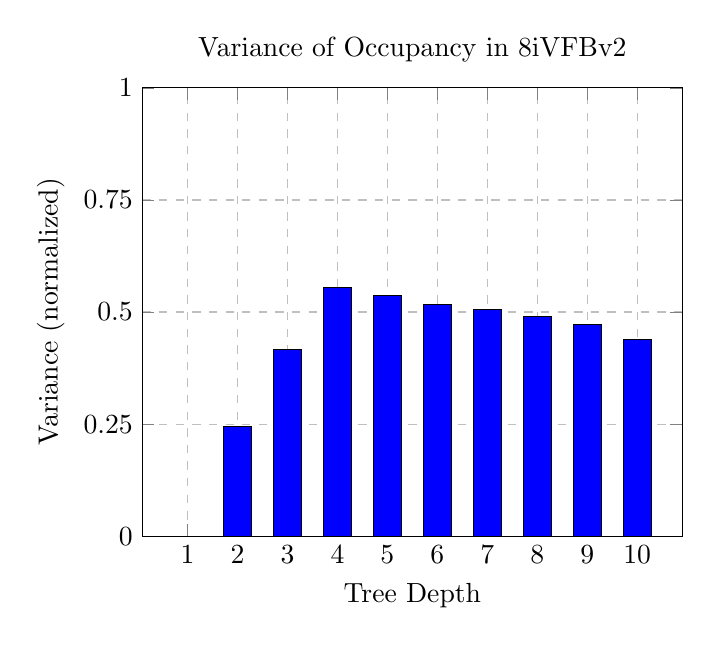
\begin{tikzpicture}
\begin{axis}[
    title={Variance of Occupancy in 8iVFBv2},
    xlabel={Tree Depth},
    ylabel={Variance (normalized)},
    symbolic x coords={1,2,3,4,5,6,7,8,9,10},
    xtick=data,
    ymin=0, ymax=1.0,
    ytick={0.0,0.25,0.5,0.75,1.0},
    xmajorgrids=true,
    ymajorgrids=true,
    grid style=dashed,
]

\addplot[
    ybar,
    fill=blue
]
coordinates {
    (1, 0.0)
    (2, 0.24456905)
    (3, 0.41581164)
    (4, 0.55556464)
    (5, 0.53706259)
    (6, 0.5164308)
    (7, 0.50496453)
    (8, 0.49014243)
    (9, 0.47307183)
    (10, 0.43909567)
};    
\end{axis}
\end{tikzpicture}
}
%\end{adjustwidth}

%\isPreprints{}{% This command is only used for ``preprints''.
%\end{adjustwidth}
%} % If the paper is ``preprints'', please uncomment this parenthesis.
\caption{
Variance in occupancy distributions across octree levels.
(\textbf{a}) SemanticKITTI (sparse): entropy is low at shallow and deep levels, but peaks at mid-levels where structural variation is highest.
(\textbf{b})~8iVFBv2 (dense): occupancy distributions maintain consistently high variance starting from level 4 due to dense and surface-complete geometry.}
\label{fig:variance_plot}
\end{figure} 

In principle, each octree level could be processed by an individually parameterized sub-module with dedicated convolutional and dense layers, enabling optimal adaptation to its entropy profile.
However, such a design is computationally expensive, memory-intensive, and reduces parameter sharing, which may impair generalization.
To balance expressiveness and efficiency, we group neighboring octree levels into a limited number of sub-modules, each tailored to a characteristic entropy regime, as follows:

\begin{itemize}
    \item Module A (Shallow Levels): Processes the coarsest levels, where occupancy is dense and entropy is low.
    A compact configuration with fewer parameters is sufficient, as occupancy patterns are highly predictable.
  
    \item Module B (Intermediate Levels): Covers the layers with the greatest variability in occupancy and the highest entropy.
    Here, a more expressive representation is required.
    Since spatial structure is still relatively coarse, increasing the channel dimension $k$ is more effective than increasing the number of layers $N$.
  
    \item Module C (Deep Levels): Handles the finest levels, where occupancy is sparse and spatial geometry must be inferred from broader context.
    In this regime, a large receptive field is essential, favoring a higher depth $N$ of convolutional layers to propagate long-range dependencies.
\end{itemize}

This level-wise grouping strategy preserves predictive accuracy across the entire octree depth while controlling computational cost, enabling efficient modeling of both coarse global structure and fine-grained geometric detail.
Moreover, the modular decomposition allows individual sub-modules to be fine-tuned, replaced, reused, or extended independently, facilitating adaptation of the codec to different application requirements such as memory constraints, target resolution, or operational latency.

\section{Experiments}
\label{sec:experiments}

This section outlines the experimental setup used to evaluate the proposed MIC-OPCCv2 framework, including datasets, implementation details, and evaluation metrics.
We then compare our method against representative state-of-the-art \acrshort{pcgc} approaches on both sparse and dense benchmarks.

\subsection{Datasets}
\label{sec:datasets}

To verify the robustness of \acrshort{MIC-OPCC}v2 across different geometric structures, we evaluate the model on both sparse and dense point cloud datasets. For fair comparison, we adopt the same training and test splits as previous studies~\citep{ECM-OPCC}.

\subsubsection{SemanticKITTI}
The SemanticKITTI dataset~\citep{SemanticKITTI} consists of large-scale outdoor LiDAR scans captured from a rotating 64-beam sensor at 10~Hz. Each frame contains roughly $10^5$ points with coordinates $\mathbf{p}=(x,y,z,l)$, where the intensity $l$ is not considered in our experiments.
The point clouds are stored in 32-bit floating-point precision with a spatial resolution of $10^{-4}$ meters and span up to approximately 270~m in diameter, requiring 18 bits per coordinate for lossless quantization.
Following the standard protocol, sequences 00--10 are used for training, while the remaining sequences serve for testing.

\subsubsection{MPEG's 8i Voxelized Full Bodies (8iVFBv2)}
The 8iVFBv2 dataset~\citep{8iVFBv2} is used to evaluate performance on dense point clouds composed of voxelized human scans.
Although the dataset contains both geometry and color, only geometry is considered in this work.
The dataset is widely adopted due to its standardized quantization levels (10--12 bits), enabling controlled \acrshort{rd} comparisons. Following common practice~\citep{MPEG}, we evaluate four benchmark sequences: \textit{Redandblack} and \textit{Loot} (300 frames each), as well as single frames from \textit{Thaidancer} and \textit{Boxer}, while \textit{Longdress} and \textit{Soldier} are used for training.

\subsection{Implementation Details}
\label{sec:implementation_details}

MIC-OPCCv2 is implemented in \texttt{TensorFlow 2.9} by using \texttt{Python 3.6} and an integrated arithmetic coder \texttt{TensorFlow Compression 2.9} provided by Ball{\'{e}}~{et al.}~\citep{TFRangeCoder}.
We configure two model variants (as illustrated in Figure~\ref{fig:model_config}): one optimized for sparse point clouds and one for dense point clouds.

\vspace{-12pt}

\begin{figure}[H]
%\begin{adjustwidth}{-\extralength}{0cm}
%\centering
\subfloat[\centering]{\includegraphics[width=0.45\textwidth]{mic-opcc/figures/SparseModel.pdf}}\hspace{-6pt}
\hfill
\subfloat[\centering]{\includegraphics[width=0.45\textwidth]{mic-opcc/figures/DenseModel.pdf}}
%\end{adjustwidth}
\caption{Model configurations for sparse and dense point clouds.
(\textbf{a}) The sparse configuration employs four sub-modules, each with a distinct number of blender layers $N$ and kernel size $k$, reflecting the varying entropy across octree depths in sparse point clouds.
(\textbf{b}) The dense configuration assumes a more uniform occupancy distribution, using five sub-modules with fixed kernel size and gradually increasing depth to accommodate consistently high spatial detail.
}
\label{fig:model_config}
\end{figure}
The \textit{sparse model} supports a quantization precision of up to $L=12$ and is divided into four sub-modules (Section~\ref{sec:model_splitting}), with each sub-module responsible for three octree levels.
These sub-modules use $N=[3,6,9,12]$ blender layers and kernel sizes $k=[16,32,64,48]$, respectively.
The total number of trainable parameters remains below one million, and the memory footprint during decoding does not exceed $2$\,KB per point.

The \textit{dense model} supports a quantization precision of up to $L=10$ and is composed of five sub-modules, each covering two octree levels.
Here, the sub-modules use $N=[2,4,6,8,10]$ blender layers with a constant kernel size of $k=64$.
This configuration results in approximately $1.4$~M trainable parameters, and the memory footprint during decoding remains below $4$~KB per point.

\subsection{Training Details}
\label{sec:training_details}

\textls[-15]{Both model variants are trained on single NVIDIA RTX~3090 GPU with 24~GB VRAM for approximately 30 epochs using the ADAM~\citep{ADAM} optimizer, an initial learning rate of $10^{-4}$ with exponential decay ($0.9$), and a dropout rate of $0.01$ to mitigate overfitting.
The loss function follows Equation~\eqref{eq:loss}, computed over all octree levels and autoregressive groups.
The final training accuracies reach about 88\% (sparse) and 94\% (dense) for occupancy~prediction.}

\subsection{Baseline}
\label{sec:baseline}

We compare \acrshort{MIC-OPCC}v2 against representative traditional and neural point cloud geometry compression methods, including
G-PCCv14~\citep{G-PCC}, VoxelContextNet~\citep{VoxelContextNet}, SparseVoxelDNN~\citep{SparseVoxelDNN}, SparsePCGCv2~\citep{SparsePCGC}, UniPCGC~\citep{UniPCGC}, RENO~\citep{RENO}, EHEM~\citep{EHEM}, and ECM-OPCC~\citep{ECM-OPCC}.
Methods that are either superseded by more recent variants or consistently underperform traditional codecs are omitted.
Furthermore, approaches such as MuSCLE~\citep{MuSCLE}, RIDDLE~\citep{RIDDLE}, and MLEM-LPCC~\citep{MLEM-LPCC}, which rely on latent feature reconstruction and therefore operate under a different compression paradigm, are excluded as well to maintain fair comparison.

\subsection{Evaluation Metrics}
\label{sec:evaluation_metrics}

We follow \acrshort{MPEG} standard evaluation procedures~\citep{MPEG} and report the following:

\begin{itemize}
    \item Bits per point (bpp): average coding cost per point.
    \item D1-PSNR (dB): point-to-point \acrshort{psnr} for geometric reconstruction fidelity.
    \item D2-PSNR (dB): point-to-plane \acrshort{psnr} for surface reconstruction fidelity.
    \item BD-Rate (\%): Bjøntegaard delta bitrate relative to a reference model~\citep{BD-Rate}.
    \item Runtime (s/frame): wall-clock encoding and decoding time.
\end{itemize}

For sparse compression on SemanticKITTI, we evaluate \acrshort{rd} using
\begin{gather}
\text{D1-PSNR} = 10\log_{10}\frac{3p^2}{\text{MSE}_{sym}}, \\
\text{MSE}_{sym} = \frac{1}{2}\left(\text{MSE}(P,\hat P)+\text{MSE}(\hat P,P)\right),
\end{gather}
where
\begin{gather}
\text{MSE}(P, \hat P) = \frac{1}{|P|}\sum_{i}\min_j\lvert \mathbf{p}_i-\mathbf{\hat p}_j\rvert^2,
\end{gather}
and the point-to-plane version uses
\begin{gather}
\text{MSE}_\mathbf{n}(P, \hat P) = \frac{1}{|P|}\sum_{i}\min_j|\mathbf{n}_i(\mathbf{p}_i-\mathbf{\hat p}_j)|^2
\end{gather}
where $\mathbf{n}_i$ is the normal-vector for $\mathbf{p}_i$.

For lossless dense compression, we report \acrshort{BD-Rate} relative to G-PCCv14.

\section{Results}
\label{sec:results}

Figure~\ref{fig:kitti_plot} illustrates the \acrshort{rd} of \acrshort{MIC-OPCC}v2 on the SemanticKITTI dataset.
With a quantization precision of $L=12$, our method achieves a bitrate of 3.41~bpp at a D2-\acrshort{psnr} of 82~dB, matching \acrshort{ECM-OPCC} and thereby approaching the current state-of-the-art for sparse point cloud geometry compression.
\vspace{-12pt}

\pgfplotsset{
    width=\textwidth*0.5,
    tick label style={font=\footnotesize},
    label style={font=\small},
    legend style={font=\tiny},
}
% Example of a figure that spans the whole page width and with subfigures. The same concept works for tables, too.
\begin{figure}[H]
%\isPreprints{}{% This command is only used for ``preprints''.
%\begin{adjustwidth}{-\extralength}{0cm}
%\centering
%} % If the paper is ``preprints'', please uncomment this parenthesis.
\subfloat[\centering]{
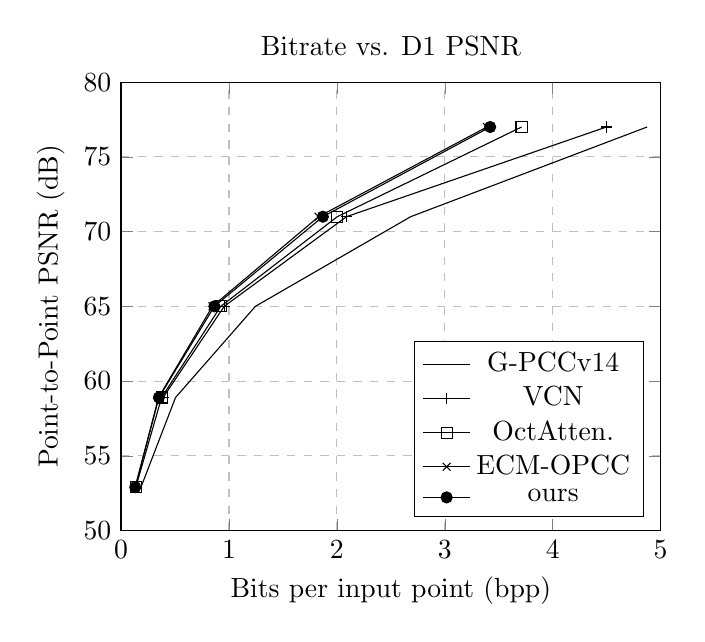
\begin{tikzpicture}
\begin{axis}[
    title={Bitrate vs. D1 PSNR},
    xlabel={Bits per input point (bpp)},
    ylabel={Point-to-Point PSNR (dB)},
    xmin=0, xmax=5,
    ymin=50, ymax=80,
    xtick={0,1,2,3,4,5},
    ytick={50,55,60,65,70,75,80},
    legend pos=south east,
    xmajorgrids=true,
    ymajorgrids=true,
    grid style=dashed,
]

\addplot[
    color=black
]
coordinates {
    (0.185,52.9)(0.505,58.9)(1.245,65.0)(2.684,71.0)(4.874,77.0)
};
\addlegendentry{G-PCCv14}

\addplot[
    color=black,
    mark=+,
]
coordinates {
   (0.390,58.9)(0.956,65.0)(2.089,71.0)(4.497,77.0)
};
\addlegendentry{VCN}

\addplot[
    color=black,
    mark=square,
]
coordinates {
    (0.137,52.9)(0.376,58.9)(0.924,65.0)(2.004,71.0)(3.711,77.0)
};
\addlegendentry{OctAtten.}

\addplot[
    color=black,
    mark=x,
]
coordinates {
    (0.131,52.9)(0.348,58.9)(0.847,65.0)(1.831,71.0)(3.39,77.0)
};
\addlegendentry{ECM-OPCC}

\addplot[
    color=black,
    mark=*,
]
coordinates {
    (0.132,52.9)(0.351,58.9)(0.865,65.0)(1.87,71.0)(3.42,77.0)
};
\addlegendentry{ours}
    
\end{axis}
\end{tikzpicture}
}
\hfill
\subfloat[\centering]{
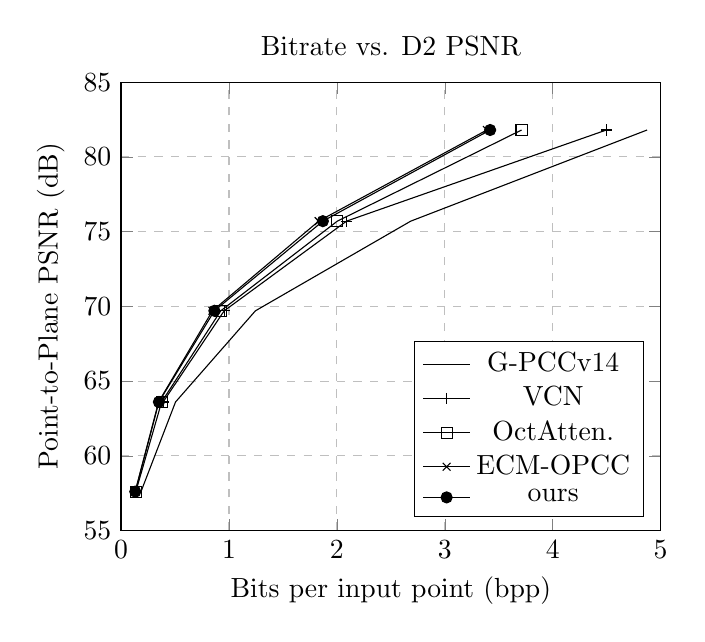
\begin{tikzpicture}
\begin{axis}[
    title={Bitrate vs. D2 PSNR},
    xlabel={Bits per input point (bpp)},
    ylabel={Point-to-Plane PSNR (dB)},
    xmin=0, xmax=5,
    ymin=55, ymax=85,
    xtick={0,1,2,3,4,5},
    ytick={55,60,65,70,75,80,85},
    legend pos=south east,
    xmajorgrids=true,
    ymajorgrids=true,
    grid style=dashed,
]

\addplot[
    color=black
]
coordinates {
    (0.185,57.6)(0.505,63.6)(1.245,69.7)(2.684,75.7)(4.874,81.8)
};
\addlegendentry{G-PCCv14}

\addplot[
    color=black,
    mark=+,
]
coordinates {
   (0.390,63.6)(0.956,69.7)(2.089,75.7)(4.497,81.8)
};
\addlegendentry{VCN}

\addplot[
    color=black,
    mark=square,
]
coordinates {
    (0.137,57.6)(0.376,63.6)(0.924,69.7)(2.004,75.7)(3.711,81.8)
};
\addlegendentry{OctAtten.}

\addplot[
    color=black,
    mark=x,
]
coordinates {
    (0.131,57.6)(0.348,63.6)(0.847,69.7)(1.831,75.7)(3.39,81.8)
};
\addlegendentry{ECM-OPCC}

\addplot[
    color=black,
    mark=*,
]
coordinates {
    (0.132,57.6)(0.351,63.6)(0.865,69.7)(1.87,75.7)(3.42,81.8)
};
\addlegendentry{ours}
    
\end{axis}
\end{tikzpicture}
}

%MDPI: Please note that each subfigure should be described separately in the caption., e.g., (a) xxx; (b) xxx.
%AUTHORS: Thank you, captions have been added.
\caption{
Results of our proposed MIC-OPCC model against state-of-the-art baselines on the SemanticKITTI dataset. While achieving comparable compression ratios to OctAttention, our model significantly outperforms it in both encoding and decoding speed. (\textbf{a}) shows the point-to-point distortion, and (\textbf{b}) the point-to-plane distortion.
\label{fig:kitti_plot}
}
\end{figure} 

VoxelContextNet, SparsePCGCv2, and \acrshort{ECM-OPCC} all employ identical quantization strategies, allowing direct comparison of their \acrshort{psnr} values.
In contrast, \acrshort{RENO} and \acrshort{EHEM} assume a peak signal of $p=59.7$ and apply different quantization configurations.
To ensure a fair evaluation, we normalize their \acrshort{psnr} values to $p=1$ but adopt their quantization configurations accordingly, as reflected in Table~\ref{tab:kitti_table}.
Despite not being trained at these distortion levels, \acrshort{MIC-OPCC}v2 consistently outperforms both \acrshort{RENO} and \acrshort{EHEM} in \acrshort{rd}.
This indicates that our model captures an underlying geometric representation that generalizes effectively across different resolutions, rather than relying on quantization-specific fitting.

%MDPI: Tables 2 and 4 have the duplicate captions. Please check and confirm.
%AUTHORS: Thank you, fixed.
%AUTHORS: We wish to visually separate our results from those of the baseline by a vertical line.
\begin{table}[H]
\caption{
Comparison of \acrshort{rd} performance and decoding time on the SemanticKITTI dataset under different quantization schemes.
For each baseline method, the original reported \acrshort{bpp} and runtime are compared with the corresponding results obtained using our proposed framework under identical quantization settings.
D1-PSNR is measured at $L=12$ and $p=1$.
}
\label{tab:kitti_table}
\isPreprints{\centering}{}
\begin{tabularx}{\textwidth}{lcccc|cc}
\toprule
 & \textbf{Quantization} & \textbf{D1-PSNR (dB)} & \multirowcell{2}{\textbf{bpp}} & \multirowcell{2}{\textbf{Time (s)}} & \multicolumn{2}{c}{\textbf{Ours}} \\
 & \boldmath{$L=12$} & \boldmath{$p=1$} & & & \textbf{bpp} & \textbf{Time (s)} \\
\midrule
ECM-OPCC & $\left\lfloor P\frac{2^{L}-1}{\max(P)-\min(P)} \right\rfloor$ & 77.2 & 3.39 & - & 3.41 & 4.0 \\[12pt] %22.03

EHEM & $ \left\lfloor P\frac{2^{L}-1}{400} \right\rfloor$ & 60.0 & 2.6 & 0.43 & 1.99 & 3.0 \\[12pt] %18.67

RENO & $ \left\lfloor P\frac{1000}{2^{18-L}} \right\rfloor$ & 61.8 & 2.9 & 0.05 & 2.41 & 3.6  \\ %18.00
\bottomrule
\end{tabularx}
\end{table}

Compared to MIC-OPCCv2, ECM-OPCC achieves superior compression performance on sparse point clouds mainly due to its attention-based context model, which can flexibly capture long-range and cross-level dependencies that are common in sparse geometries.
Although ECM-OPCC relies on a linear octree traversal order that does not always preserve spatial neighborhood coherence, the global receptive field of self-attention compensates for this limitation by selectively emphasizing informative occupied regions.
In contrast, MIC-OPCCv2 prioritizes decoding efficiency through structured index-based context modeling, which favors spatial coherence and linear complexity but may be less expressive in extremely sparse regimes. While ECM-OPCC could further benefit from more advanced indexing strategies, its transformer architecture incurs a significantly higher memory footprint and runtime cost, making MIC-OPCCv2 more suitable for large-scale or latency-constrained~scenarios.

For dense geometry evaluated on the 8iVFBv2 dataset, \acrshort{MIC-OPCC}v2 achieves an average bitrate of 0.50~bpp, outperforming UniPCGC and \acrshort{ECM-OPCC} by approximately $1.14\%$ and $11.2\%$ in \acrshort{BD-Rate}, respectively (see Table~\ref{tab:8iVFBv2}).
SparseVoxelDNN attains superior compression performance on this dataset, which can be attributed to its fully voxel-wise autoregressive modeling that exploits dense and regular occupancy patterns more exhaustively.
In contrast, \acrshort{MIC-OPCC}v2 prioritizes decoding efficiency through grouped autoregression and linear complexity, which leads to a substantially reduced decoding time.
Specifically, \acrshort{MIC-OPCC}v2 decodes a frame in approximately 5 s, making it roughly ${\sim}40\times$ faster than SparseVoxelDNN and ${\sim}4\times$ faster than \acrshort{ECM-OPCC}, while remaining slower than UniPCGC, which reports an average decoding time of 0.57 s per frame.

While the model achieves competitive or state-of-the-art \acrshort{rd} performance, the observed decoding latency highlights the need for further implementation-level optimization to fully exploit the theoretical efficiency of the architecture.

Overall, the results demonstrate that incorporating the progressive grouping strategy markedly enhances the effectiveness of multi-index convolution.
\acrshort{MIC-OPCC}v2 surpasses every baseline model in at least one of the two key performance dimensions: bitrate efficiency or decoding speed.
This indicates that the model generalizes well across both sparse and dense point cloud distributions, achieving competitive or state-of-the-art \acrshort{rd}.
However, the current decoding latency suggests that additional engineering optimizations are still needed to fully realize the theoretical efficiency of the proposed architecture.

%MDPI: Please confirm if the bold formatting is necessary; if not, please remove it. The following highlights are the same.
%AUTHORS: These are table headers in the left column.
%AUTHORS: We find, headers in top row AND very left column should be bold. Remove it if this is a format violation.
%AUTHORS: Note that there are names of data samples (normal) and metric headers (bold)!
\begin{table}[H]
\caption{Average compression ratio (bpp) of 8iVFBv2, showing the gain over G-PCCv14 and coding~time.}
\label{tab:8iVFBv2}
%\isPreprints{\centering}{}
\tabcolsep=0.557cm
\begin{adjustwidth}{-\extralength}{0cm}
%\centering %% If there is a figure in wide page, please release command \centering, for Table, ``\textwidth" should be ``\fulllength"
\begin{tabular}{lccccc}

\toprule
\textbf{Point Clouds} & \textbf{GPCC} & \textbf{MIC-OPCCv2} & \textbf{UniPCGC}   & \textbf{SparseVoxelDNN} & \textbf{ECM-OPCC} \\
\midrule
Redandblack           & 0.82         & 0.57              & 0.59              & 0.41                   & 0.66         \\
Loot                  & 0.69         & 0.48              & 0.49              & 0.32                   & 0.55         \\
Thaidancer            & 0.70         & 0.50              & 0.51              & 0.33                   & 0.58         \\
Boxer                 & 0.65         & 0.43              & 0.45              & 0.30                   & 0.51         \\
\midrule
\textbf{Average Bpp}  & 0.72         & 0.50              & 0.51              & 0.34                   & 0.58         \\
\textbf{Gain$^{-1}$}  & 0.0\%        & 30.6\%            & 29.2\%            & 52.8\%                 & 19.4\%      \\
\midrule
\textbf{Enc time(s)}  & 1.99         & 5.0               & 0.56              & 7.2                    & 1.92         \\
\textbf{Dec time(s)}  & 1.49         & 5.0               & 0.57              & 229                    & 19.5         \\
\midrule
\textbf{Test Device} & i7           & RTX3090           & RTX4080           & RTX3090                & RTX3090      \\
\bottomrule

\end{tabular}
\end{adjustwidth}
\end{table}

\section{Discussion}
\label{sec:discussion}

The experimental results from Section~\ref{sec:results} demonstrate that \acrshort{MIC-OPCC}v2 effectively bridges the gap between sparse convolutional and transformer-based PCGC models.
By eliminating the attention overhead while preserving long-range context through multi-index convolution, the method achieves a favorable trade-off between \acrshort{rd} and computational efficiency.
Moreover, its grouping scheme enables flexible decoding parallelism, bringing it closer to real-world applications, but still struggles with real-time performance due to implementation issues.

We discuss the latency problem by analyzing the theoretical runtime complexity in the following Section~\ref{sec:runtime_complexity}.
Furthermore, in Section~\ref{sec:parceptive_field}, we demonstrate and illustrate how the perceptive field of multi-index convolution expands in sparse and dense point clouds differently, to discuss strength and weakness of our methods, that may leave room for future investigation and improvement.
To quantify the contribution of each proposed component, we present an ablation study in Section~\ref{sec:ablation_study}, demonstrating how voxel-wise prediction, the blender \& distiller network, and progressive grouping each incrementally improve compression efficiency.

\subsection{Runtime Complexity}
\label{sec:runtime_complexity}

The key idea of our multi-index convolution is to achieve a large receptive field in three-dimensional space while maintaining low computational complexity.
Table~\ref{tab:complexity} summarizes the theoretical complexity of transformers, Minkowski convolution, and our proposed multi-index convolution, alongside their measured decoding times.
\begin{table}[H] 
\caption{
Theoretical computational complexity of three leading point cloud compression architectures and their corresponding practical decoding times.
\label{tab:complexity}
}
%\centering
\begin{tabularx}{\textwidth}{CCCC}
    \toprule
    \textbf{Method} & \textbf{Complexity} & \textbf{Example} & \textbf{Decoding Time (s)} \\
    \midrule
    Transformer & $\mathcal{O}\left(n(3ckw + kw^2)\right)$ & ECM-OPCC & 19.5 \\[6pt]
    Minkowski Convolution & $\mathcal{O}\left(m(ckw^d)\right)$ & UniPCGC & 0.57 \\[12pt]
    Multi-Index Convolution & $\mathcal{O}\left(n(ckwi)\right)$ & MIC-OPCCv2 & 5.0 \\
    \bottomrule
\end{tabularx}
\end{table}
%\unskip

It is evident that transformer architectures exhibit the highest computational complexity, making them the least efficient in this comparison.
For each data point $n$, a transformer requires the computation of the key, value, and query layers, contributing $3ck$, as well as the attention matrix with complexity $kw^2$, where $w$ denotes the window size, $c$ the number of input channels, and $k$ the kernel size (i.e., number of output channels).

The Minkowski convolution, as defined by Choy~C.~{et al.}~\citep{Minkowski}, generalizes the standard convolution to sparse domains, with a core complexity of $ckw^{d=3}$ that scales with the number of query points $m$.
To maintain equivalence with dense convolutional outputs, the query count $m$ increases across stacked layers due to the propagation of kernel offsets around each point $n$:
\begin{equation}
m = n \frac{(N - 1)w^d}{\epsilon},
\end{equation}
where $N$ is the number of layers and $\epsilon$ is a correction factor accounting for overlapping receptive fields.
This factor $\epsilon$ tends to be smaller for dense point clouds (due to more overlap) and larger for sparse point clouds.

\textls[-15]{In contrast, the theoretical complexity of our multi-index convolution, given by $n(ckwi)$, is substantially lower than that of Minkowski convolution, since $w(i=4) < w^{d=3}$, where $i$ denotes the number of applied index orders $I$ and $n$ remains constant.
However, despite this theoretical advantage, our current implementation exhibits a runtime roughly ten times slower than sparse Minkowski-based models.
We attribute this discrepancy to non-optimized index reordering operations (see Figure~\ref{fig:profiling}), which cause extended GPU idle periods during the rearrangement of feature vectors $F$ across index sets $I$.
Ongoing optimization efforts aim to minimize these bottlenecks and further improve practical~efficiency.}
\begin{figure}[H]
%\centering
%MDPI: The contents of this figure are not legible. Please replace the image with one of a sufficiently high resolution (min. 1000 pixels width/height, or a resolution of 300 dpi or higher).
\includegraphics[width=0.5\textwidth]{mic-opcc/figures/profiling.png}
\caption{
TensorBoard profiler pie chart illustrating the distribution of total on-device self-time by operation type (in percent). PyFunc denotes poorly supported Python operations---most notably gather and scatter routines---which account for a substantial portion of execution time and lead to idle periods on the acceleration hardware.
}
\label{fig:profiling}
\end{figure}

\subsection{Perceptive Field}
\label{sec:parceptive_field}

Figure~\ref{fig:perceptive_field} illustrates the theoretical activation score of the spatial receptive field generated by our multi-index convolution, using a Gaussian filter.
This visualization demonstrates how the proposed method effectively bridges large gaps in sparse point clouds, enabling better spatial context understanding in samples as in the SemanticKITTI dataset.
On the other hand, this method occasionally extends beyond the object's convex hull, unintentionally capturing points from the backside.
Hence, the spatial compactness of this method is not guaranteed and intuitively highlights a limitation when applied to dense or closed-surface geometries as in samples from the \acrshort{MVUB}~\citep{MVUB} dataset.
Nonetheless, we assume that the learned filters of our model should easily detect the un-similarity between these far distant voxels and lower their activation score.

\vspace{-12pt}

\begin{figure}[H]
%\begin{adjustwidth}{-\extralength}{0cm}
%MDPI: 1. Please add an explanation of subfigure (c). 2. Figure priority to put it below the first mentioned paragraph, and do Not across the section titles. However, to reduce white space, we recommend moving it across the Heading 7.3, please check and modify.
\subfloat[\centering]{\includegraphics[width=0.4\textwidth]{mic-opcc/figures/PerceptiveFieldKitti12.png}}
\subfloat[\centering]{\includegraphics[width=0.4\textwidth]{mic-opcc/figures/PerceptiveFieldMVUB.png}}
\subfloat[\centering]{\includegraphics[width=0.1\textwidth]{mic-opcc/figures/Colorscale.png}}
%\end{adjustwidth}
\caption{
Theoretical activation score of the spatial receptive field generated by our multi-index convolution.
(\textbf{a}) illustrates the receptive field on a sample from the SemanticKITTI dataset.
(\textbf{b}) illustrates the receptive field on a sample from the MVUB dataset.
(\textbf{c}) is the color scale used to illustrate the activation score.
\label{fig:perceptive_field}
}
\end{figure}
\subsection{Ablation Study}
\label{sec:ablation_study}

To better understand the contribution of each design choice in \acrshort{MIC-OPCC}v2, we conduct a comprehensive ablation study that systematically evaluates the impact of the proposed architectural components and decoding strategies.
In particular, we analyze how different autoregressive grouping schemes, depth-aware model splitting, and key module activations affect compression efficiency, estimation accuracy, memory consumption, and inference latency.
Unless stated otherwise, all ablation experiments are performed under identical training settings to ensure fair and interpretable comparisons.

%MDPI: 1. We noted that * is not included in the table body. Could you please confirm if it can be added? If not, we suggest removing it for clarity and consistency.2. Please confirm if the italics are necessary; if not, please remove them.
%AUTHORS: 1. It was there before.

Table~\ref{tab:grouping_ablation} evaluates the effect of different autoregressive grouping strategies on compression efficiency, estimation accuracy, memory consumption, and inference latency.
Decoding without grouping achieves the lowest inference time but performs poorly in terms of bitrate and accuracy, indicating insufficient contextual modeling when all octree-nodes are decoded in a single stage.
Sequential grouping substantially improves both bitrate and accuracy by enforcing strict voxel-wise autoregression per octree-node; however, this benefit comes at the cost of significantly increased inference time due to reduced parallelism.
The proposed progressive grouping strategy provides the most favorable trade-off, achieving the lowest \acrshort{bpp} and highest estimation accuracy while maintaining considerably lower inference latency than sequential grouping.
Although progressive grouping introduces a moderate increase in peak memory usage compared to sequential decoding, it remains substantially more efficient than the no-grouping baseline, demonstrating that gradually expanding the decoding scope effectively balances contextual refinement and computational efficiency.
\begin{table}[H]
\caption{
Ablation study of different autoregressive grouping strategies using the MVUB dataset~\citep{MVUB}.
Without Grouping: No voxel grouping is applied and decoding follows a fully parallel scheme. All voxel $v$ of all octree-nodes $\mathbf{o}_t$ are decoded a in single stage.
Sequential Grouping: One voxel $v_{g}$ of all octree-nodes $\mathbf{o}_{t}$ are decoded in parallel at each monotonic step $g \in [1\dots8]$.
Progressive Grouping: The proposed strategy, which skips a subset of octree-nodes during early stages ($g \leq 4$) to reduce uncertainty and progressively decodes multiple voxel candidates per node in later stages ($g > 6$) as contextual information becomes richer.
(* Peak memory spikes observed during backpropagation.)
}
\label{tab:grouping_ablation}
%\isPreprints{\centering}{}
\tabcolsep=0.595cm

\begin{adjustwidth}{-\extralength}{0cm}
%\centering %% If there is a figure in wide page, please release command \centering, for Table, ``\textwidth" should be ``\fulllength"
\begin{tabular}{lccc}

\toprule
\textbf{Method}                 & \textbf{Without Grouping} & \textbf{Sequential Grouping}  & \textbf{Progressive Grouping}  \\
\midrule
\textbf{Bits per Point}         &  1.25                 & 0.76                          & 0.64   \\
\textbf{Estimation Accuracy}    &  84\%                 & 90\%                          & 92\% \\
\textbf{Memory Peak per Point}* &  14.6 KB               & 10.1 KB                        & 12.9 KB \\
\textbf{Inference per Point}    &  1.076 ns              & 3.105 ns                       & 2.594 ns   \\
\bottomrule

\end{tabular}
\end{adjustwidth}
\end{table}


Table~\ref{tab:model_splitting_ablation} investigates the impact of progressively splitting the network into depth-specific sub-modules along the octree hierarchy.
Transitioning from a single monolithic model 0--12 to increasingly fine-grained depth splits consistently improves compression efficiency and estimation accuracy, reducing the bitrate from 4.169 to 3.715 \acrshort{bpp} while increasing accuracy from 84.2\% to 86.0\%.
At the same time, inference cost per point decreases monotonically, indicating that shallower, depth-specialized sub-modules enable more efficient computation.
Notably, improvements saturate beyond the 0--4--8--12 configuration, where further splitting yields only marginal gains while maintaining similar memory requirements.
This suggests that moderate depth-aware model splitting offers a favorable balance between compression performance, runtime efficiency, and memory~consumption.
\begin{table}[H]
\caption{
Ablation study of the proposed model-splitting strategy, where dedicated sub-modules are assigned to different depth ranges of the octree.
Table header labels denote model configurations; for example, 0--4--8--12 indicates three sub-modules split at octree layers 4, 8, and 12.
To illustrate scaling behavior, each sub-module contains a number of convolution layers equal to its upper split boundary (i.e., 4, 8, and 12 layers).
All configurations are evaluated on the SemanticKITTI dataset~\citep{SemanticKITTI} for 10~epochs with 1000 samples per epoch.
(* Peak memory spikes observed during backpropagation.) 
}
\label{tab:model_splitting_ablation}
%\isPreprints{\centering}{}
\tabcolsep=0.495cm
\begin{adjustwidth}{-\extralength}{0cm}
%\centering %% If there is a figure in wide page, please release command \centering, for Table, ``\textwidth" should be ``\fulllength"
%AUTHORS: We find, headers in top row AND very left column should be bold. Remove it if this is a format violation.
\begin{tabular}{lccccc}

\toprule
\textbf{Model Splitting} & \textbf{0--12} & \textbf{0--6--12} & \textbf{0--4--8--12} & \textbf{0--3--6--9--12} & \textbf{0--2--4--6--8--10--12} \\
\midrule
\textbf{Bits per Point} & 4.169 & 3.883 & 3.722 & 3.720 & 3.715 \\
\textbf{Estimation Accuracy} & 84.2\% & 85.3\% & 85.9\% & 86.0\% & 86.0\% \\
\textbf{Memory Peak per Point} * & 116.9 KB & 117.3 KB & 117.1 KB & 117.0 KB & 117.2 KB \\
\textbf{Inference per Point} & 0.532 ns & 0.434 ns & 0.405 ns & 0.392 ns & 0.367 ns \\
\bottomrule

\end{tabular}
\end{adjustwidth}
\end{table}


Table~\ref{tab:ablation_study} disentangles the contributions of the major components introduced in \acrshort{MIC-OPCC}v2.
Starting from the \acrshort{MIC-OPCC}v1 baseline, which performs octree-node occupancy estimation using depth-specific sub-modules, we incrementally activate each proposed design element from Section~\ref{sec:methods} and evaluate its impact relative to the G-PCCv14 anchor.
Replacing node estimation with voxel estimation yields the first substantial improvement, increasing the \acrshort{BD-Rate} gain from 20.2\% to 21.8\%, confirming that voxel-level supervision provides a more expressive learning signal for context modeling.
Introducing the blender \& distiller architecture further boosts performance to a gain of 25.4\%, highlighting the effectiveness of multi-scale residual aggregation and voting-based distillation in stabilizing predictions across each hidden layer.
Adding sequential grouping increases the gain to 28.1\% but also raises decoding time from approximately ${\sim}3$ s to over ${\sim}5$ s per frame, illustrating the latency cost of strict autoregressive decoding.
Replacing this scheme with the proposed progressive grouping strategy preserves comparable compression gains (28.6\%) while avoiding additional runtime penalties by retaining partial parallelism.
Finally, combining progressive grouping with the Sub-Module design yields the full \acrshort{MIC-OPCC}v2 model, achieving the highest gain of 30.6\% with a decoding time of approximately 5.1 s.
This configuration represents the most favorable balance between compression efficiency and computational cost among all evaluated variants.

Overall, the ablation study demonstrates that each proposed component contributes meaningfully to performance improvements.
The largest gains stem from voxel-based estimation, the blender \& distiller architecture, and the progressive grouping strategy, whose combination enables \acrshort{MIC-OPCC}v2 to substantially outperform the \acrshort{MIC-OPCC}v1 baseline while maintaining practical decoding complexity.

\begin{table}[H]
\caption{
Ablation study of the proposed methods from Section~\ref{sec:methods}. All BD-Rates are relative to G-PCCv14.
A checkmark (\checkmark) indicates that the corresponding method is enabled in the evaluated configuration.
}
\label{tab:ablation_study}
%\isPreprints{\centering}{}
\tabcolsep=0.155cm
%\begin{adjustwidth}{-\extralength}{0cm}
%\centering %% If there is a figure in wide page, please release command \centering, for Table, ``\textwidth" should be ``\fulllength"
%MDPI: Please confirm whether an explanation of the \checkmark needs to be added to the table footer.
%AUTHORS: Checkmarks are now explained
%AUTHORS: We find, headers in top row AND very left column should be bold. Remove it if this is a format violation.

\begin{tabular}{lcccccc}
\toprule
\textbf{Method}                 & \textbf{MIC-OPCCv1}   &            &            &            &            & \textbf{MIC-OPCCv2}  \\
\midrule
\textbf{node estimation}        & \checkmark            &            &            &            &            &            \\
\textbf{voxel estimation}       &                       & \checkmark & \checkmark & \checkmark & \checkmark & \checkmark \\
\textbf{Blender \& Distiller}   &                       &            & \checkmark & \checkmark & \checkmark & \checkmark \\
\textbf{Sequential Grouping}    &                       &            &            & \checkmark &            &            \\
\textbf{Progressive Grouping}   &                       &            &            &            & \checkmark & \checkmark \\
\textbf{Sub-Modules}            & \checkmark            &            &            &            &            & \checkmark \\
\midrule
\textbf{Gain$^{-1}$}            & 20.2\%                & 21.8\%     &  25.4\%    &  28.1\%    &  28.6\%    & 30.6\%     \\
\textbf{Decoding Time (s)}      & 2.2                   & 2.8        &  2.9       &  5.4       &  5.3       & 5.1        \\
\bottomrule

\end{tabular}
%\end{adjustwidth}
\end{table}

\section{Conclusions and Future Work}
\label{sec:conclusion}

This paper presented \acrshort{MIC-OPCC}v2, a neural entropy model for octree-based point cloud geometry compression that addresses the long-standing trade-off between \acrshort{rd} performance and decoding latency.
By introducing multi-index convolution as a lightweight alternative to transformer-based attention and full 3D sparse convolution, the proposed framework enables explicit yet computationally efficient context modeling using only one-dimensional operations.
Combined with the blender \& distiller architecture and progressive grouping strategy, \acrshort{MIC-OPCC}v2 achieves competitive compression efficiency while substantially reducing decoding complexity and memory overhead.

Experimental results demonstrate that \acrshort{MIC-OPCC}v2 consistently outperforms traditional codecs such as G-PCC and achieves favorable \acrshort{rd} performance compared to recent neural approaches, including \acrshort{UniPCGC} and \acrshort{ECM-OPCC}, while offering up to a fourfold decoding speedup.
The method generalizes effectively across heterogeneous data regimes, ranging from sparse LiDAR scans to dense surface reconstructions.
At the same time, our results reveal a performance gap on highly dense and regular geometry when compared to fully autoregressive voxel-wise models such as SparseVoxelDNN.
This gap can be attributed to the strict voxel-level dependency modeling employed by fully autoregressive methods, which is particularly effective for dense occupancy patterns but comes at the cost of substantially higher decoding latency and memory consumption.
In contrast, \acrshort{MIC-OPCC}v2 deliberately trades a small loss in compression efficiency for significantly improved runtime scalability, making it more suitable for latency-sensitive applications.

Further analysis indicates that the advantages of multi-index convolution are most pronounced in sparse-to-moderately dense point clouds, where explicit spatial indexing provides robust contextual cues while avoiding the non-local interactions and high memory footprint inherent in attention-based models.
For highly regular dense surfaces, the fixed indexing scheme may introduce non-local voxel activations inside the perceptive field, which can limit achievable compression gains.
Similarly, while progressive grouping---following principles previously explored in \acrshort{UniPCGC}~\citep{UniPCGC}---effectively balances contextual refinement and parallelism, more adaptive grouping schedules may further improve robustness across varying data distributions.
These observations define clear applicability boundaries of the proposed approach and motivate future research directions.

Several directions remain open for future work.
First, replacing fixed index permutations with learned or data-adaptive indexing strategies may improve spatial coherence and suppress non-local activations, particularly on dense and regular geometry.
Second, more flexible grouping strategies, potentially driven by local occupancy statistics, could further optimize the \acrshort{rd} trade-off.
Third, extending the framework to jointly compress geometry and attributes such as color, reflectance, or semantic labels would enable a unified neural point cloud codec.
Finally, hardware-aware optimizations---including optimized gather/scatter primitives, quantization-aware training, and sparse acceleration---could further narrow the gap between theoretical and practical runtime performance.

In conclusion, \acrshort{MIC-OPCC}v2 demonstrates that carefully designed index-based convolutional context models can achieve a favorable balance between compression efficiency, decoding speed, and scalability.
Rather than maximizing compression performance at all costs, the proposed method explicitly targets practical deployment constraints, providing an effective and computationally tractable solution for next-generation point cloud transmission and storage.


%%%%%%%%%%%%%%%%%%%%%%%%%%%%%%%%%%%%%%%%%%
\vspace{6pt} 

%%%%%%%%%%%%%%%%%%%%%%%%%%%%%%%%%%%%%%%%%%
\authorcontributions{
Conceptualization, G.B.;
methodology, G.B.;
software, G.B.;
validation, G.B.,
formal analysis, G.B.;
investigation, G.B.;
resources, J-I.G.;
data curation, G.B.;
writing---original draft preparation, G.B.;
writing---review and editing, G.B. and J-I.G.;
visualization, G.B.;
supervision, J-I.G.;
project administration, J-I.G.;
funding acquisition, J-I.G.;
All authors have read and agreed to the published version of the manuscript.
}
%MDPI: For research articles with several authors, a short paragraph specifying their individual contributions must be provided. The following statements should be used ``Conceptualization, X.X. and Y.Y.; methodology, X.X.; software, X.X.; validation, X.X., Y.Y. and Z.Z.; formal analysis, X.X.; investigation, X.X.; resources, X.X.; data curation, X.X.; writing---original draft preparation, X.X.; writing---review and editing, X.X.; visualization, X.X.; supervision, X.X.; project administration, X.X.; funding acquisition, Y.Y. All authors have read and agreed to the published version of the manuscript.'', please turn to the  \href{http://img.mdpi.org/data/contributor-role-instruction.pdf}{CRediT taxonomy} for the term explanation. Authorship must be limited to those who have contributed substantially to the work~reported.
%AUTHORS: added

\funding{
This work is financially supported in part (project number: 115UC5N006) by
the Co-creation Platform of the Industry Academia Innovation School, NYCU, under
the framework of the National Key Fields Industry--University Cooperation and
Skilled Personnel Training Act, from the Ministry of Education (MOE) and industry
partners in Taiwan. This work is also supported in part by the National Science and
Technology Council (NSTC), Taiwan R.O.C. projects with grants 114-2218-E-002-007,
114-2640-E-A49-015, 114-2218-E-002-007, 114-2218-E-A49-020, 114-2218-E-A49-
162-MY3, 114-2218-E-A49-168-MY3, 114-2640-E-A49-017, and 114-2634-F-A49-004.
}

%MDPI: Please provide the date you accessed the URL in the following format: “URL (accessed on Day Month Year)”.
\dataavailability{Source code and pre-trained models are published on \url{https://github.com/bugerry87/mic-opcc} (accessed on 13 February 2026).} 

%\acknowledgments{}

\conflictsofinterest{The authors declare no conflicts of interest.} 

%%%%%%%%%%%%%%%%%%%%%%%%%%%%%%%%%%%%%%%%%%
%% Optional

%% Only for journal Encyclopedia
%\entrylink{The Link to this entry published on the encyclopedia platform.}

%\abbreviations{Abbreviations}{
%The following abbreviations are used in this manuscript:
%\\
%\noindent 
%\begin{tabular}{@{}ll}
%PCGC & Point Cloud Geometry Compression \\
%\end{tabular}
\newpage
\abbreviations{Abbreviations}{
\noindent 
\begin{tabular}{@{}ll}
BAC & Binary Arithmetic Coder \\
BD-Rate & Bjøntegaard Delta Rate \\
bpp & Bit Per (input) Points \\
ECM-OPCC & Efficient Context Model for Octree-based Point Cloud Compression \\
EHEM & Efficient Hierarchical Entropy Model for Learned Point Cloud Compression \\
FOC & Fast Octree Coding \\
G-PCC & Geometry-based Point Cloud Compression \\
MIC-OPCC & Multi-Index Convolution for Octree-based Point Cloud Compression \\
MLP & Multi-Layer Perceptron \\
MPEG & Moving Picture Experts Group \\
MVUB & Microsoft's Voxelized Upper Bodies \\
NNOC & \makecell[l]{Neural Network Modeling of Probabilities for Coding the Octree Representation of\\ Point Clouds} \\
PCGC & Point Cloud Geometry Compression \\
PSNR & Peak Signal-to-Noise Ratio \\
R--D & Rate--Distortion \\
RENO & Real-Time Neural Compression for 3D LiDAR Point Clouds \\
RIDDLE & Lidar Data Compression with Range Image Deep Delta Encoding \\
UniPCGC & \textls[-30]{Towards Practical Point Cloud Geometry Compression via an Efficient Unified Approach} \\
V-PCC & Video-based Point Cloud Compression \\
\end{tabular}
}

%\setlength{\glsdescwidth}{0.8\textwidth}
%\setlength{\LTleft}{-5pt}
%\printnoidxglossary[
%title=Abbreviations,
%type=\acronymtype,
%style=long,
%nogroupskip,
%nonumberlist,
%nopostdot,
%]

\begin{adjustwidth}{-\extralength}{0cm}
%%%%%%%%%%%%%%%%%%%%%%%%%%%%%%%%%%%%%%%%%%
%\begin{adjustwidth}{-\extralength}{0cm} % This command is only used for ``preprints''.
\reftitle{References}

% Please provide either the correct journal abbreviation (e.g. according to the “List of Title Word Abbreviations” http://www.issn.org/services/online-services/access-to-the-ltwa/) or the full name of the journal.
% Citations and References in Supplementary files are permitted provided that they also appear in the reference list here. 

%=====================================
% References, variant A: external bibliography
%=====================================
\begin{thebibliography}{999}

%MDPI: Newly added  information. Please confirm. The following highlights are the same.
\bibitem[Meng and Lu(2024)]{Survey1}
Meng, H.; Lu, H.
\newblock A Survey of Deep Learning Technology in Visual SLAM.
\newblock In Proceedings of the 2024 International Wireless Communications and Mobile Computing (IWCMC), Ayia Napa, Cyprus, 27--31 May 2024; pp. 37--42.
\newblock {\url{https://doi.org/10.1109/IWCMC61514.2024.10592584}}.
%MDPI: Please check whether the page number should be changed to 37--42.

\bibitem[Bhattacharyya and Kim(2023)]{Survey2}
Bhattacharyya, C.; Kim, S.
\newblock Survey and Performance Analysis on Point Cloud Classification Models.
\newblock In Proceedings of the 2023 23rd International Conference on Control,
  Automation and Systems (ICCAS), Yeosu, Republic of Korea, 17--20 October 2023; pp.~254--258.
\newblock {\url{https://doi.org/10.23919/ICCAS59377.2023.10316922}}.

\bibitem[Roriz et~al.(2024)Roriz, Silva, Dias, and Gomes]{Survey3}
Roriz, R.; Silva, H.; Dias, F.; Gomes, T.
\newblock A Survey on Data Compression Techniques for Automotive LiDAR Point
  Clouds.
\newblock {\em Sensors} {\bf 2024}, {\em 24}(10), 3185.
\newblock {\url{https://doi.org/10.3390/s24103185}}.

\bibitem[Google(2017)]{Draco}
Google.
\newblock Draco 3D Graphics Compression. 2017.
\newblock Available online: \url{https://github.com/google/draco}.
\newblock accessed: 13 February 2026

\bibitem[Li et~al.(2024)Li, Gao, and Gao]{G-PCC}
Li, G.; Gao, W.; Gao, W., MPEG Geometry-Based Point Cloud Compression (G-PCC)
  Standard.
\newblock In {\em Point Cloud Compression: Technologies and Standardization};
  Springer Nature Singapore: Singapore,  2024; pp. 135--165.
\newblock {\url{https://doi.org/10.1007/978-981-97-1957-0_7}}.

\bibitem[Nguyen et~al.(2021{\natexlab{a}})Nguyen, Quach, Valenzise, and
  Duhamel]{VoxelDNN}
Nguyen, D.T.; Quach, M.; Valenzise, G.; Duhamel, P.
\newblock Learning-Based Lossless Compression of 3D Point Cloud Geometry.
\newblock In Proceedings of the ICASSP 2021---2021 IEEE International
  Conference on Acoustics, Speech and Signal Processing (ICASSP), Toronto, ON, Canada,  6--11 June 2021; pp.
  4220--4224.
\newblock {\url{https://doi.org/10.1109/ICASSP39728.2021.9414763}}.

\bibitem[Nguyen et~al.(2021{\natexlab{b}})Nguyen, Quach, Valenzise, and
  Duhamel]{MSVoxelDNN}
Nguyen, D.T.; Quach, M.; Valenzise, G.; Duhamel, P.
\newblock Multiscale deep context modeling for lossless point cloud geometry
  compression.
\newblock In Proceedings of the 2021 IEEE International Conference on
  Multimedia Expo Workshops (ICMEW), Shenzhen, China, 5--9 July 2021; pp. 1--6.
\newblock {\url{https://doi.org/10.1109/ICMEW53276.2021.9455990}}.

\bibitem[Wang et~al.(2021)Wang, Ding, Li, Feng, Cao, and Ma]{SparsePCGC}
Wang, J.; Ding, D.; Li, Z.; Feng, X.; Cao, C.; Ma, Z.
\newblock Sparse {T}ensor-based Multiscale Representation for Point Cloud Geometry Compression.
\newblock In IEEE Transactions on Pattern Analysis and Machine Intelligence, vol. 45, no. 7, pp. 9055-9071, 1 July 2023, doi: 10.1109/TPAMI.2022.3225816.
\newblock {\url{https://doi.org/10.1109/TPAMI.2022.3225816}}.

\bibitem[Wang and Gao(2025)]{UniPCGC}
Wang, K.; Gao, W.
\newblock UniPCGC: Towards Practical Point Cloud Geometry Compression via an
  Efficient Unified Approach.
\newblock {\em Proc. AAAI Conf. Artif. Intell.}
  {\bf 2025}, {\em 39},~12721--12729.
\newblock {\url{https://doi.org/10.1609/aaai.v39i12.33387}}.

\bibitem[Huang et~al.(2020)Huang, Wang, Wong, Liu, and Urtasun]{OctSqueeze}
Huang, L.; Wang, S.; Wong, K.; Liu, J.; Urtasun, R.
\newblock Oct{S}queeze: Octree-Structured Entropy Model for LiDAR Compression.
\newblock In Proceedings of the 2020 IEEE/CVF Conference on Computer Vision and Pattern Recognition (CVPR), Seattle, WA, USA, 13--19 June 2020; pp. 1310--1320.
\newblock {\url{https://doi.org/10.1109/CVPR42600.2020.00139}}.

\bibitem[Fu et~al.(2022)Fu, Li, Song, Gao, and Liu]{OctAttention}
Fu, C.; Li, G.; Song, R.; Gao, W.; Liu, S.
\newblock Oct{A}ttention: Octree-Based Large-Scale Contexts Model for Point
  Cloud Compression.
\newblock {\em Proc. AAAI Conf. Artif. Intell.}
  {\bf 2022}, {\em 36},~625--633.
\newblock {\url{https://doi.org/10.1609/aaai.v36i1.19942}}.

\bibitem[Jin et~al.(2024)Jin, Zhu, Xu, Lin, and Wang]{ECM-OPCC}
Jin, Y.; Zhu, Z.; Xu, T.; Lin, Y.; Wang, Y.
\newblock ECM-OPCC: Efficient Context Model for Octree-Based Point Cloud
  Compression.
\newblock In Proceedings of the ICASSP 2024---2024 IEEE International
  Conference on Acoustics, Speech and Signal Processing (ICASSP), Seoul, Republic of Korea, 14--19 April 2024; pp.
  7985--7989.
\newblock {\url{https://doi.org/10.1109/ICASSP48485.2024.10446374}}.

\bibitem[Song et~al.(2023)Song, Fu, Liu, and Li]{EHEM}
Song, R.; Fu, C.; Liu, S.; Li, G.
\newblock Efficient Hierarchical Entropy Model for Learned Point Cloud
  Compression.
\newblock In Proceedings of the 2023 IEEE/CVF Conference on Computer Vision and
  Pattern Recognition (CVPR), Vancouver, BC, Canada, 17--24 June 2023; pp. 14368--14377.
\newblock {\url{https://doi.org/10.1109/CVPR52729.2023.01381}}.

\bibitem[Que et~al.(2021)Que, Lu, and Xu]{VoxelContextNet}
Que, Z.; Lu, G.; Xu, D.
\newblock Voxel{C}ontext-{N}et: An Octree Based Framework for Point Cloud
  Compression.
\newblock In Proceedings of the  IEEE/CVF Conference on
  Computer Vision and Pattern Recognition (CVPR), Nashville, TN, USA, 20--25 June 2021 ; pp. 6042--6051.

\bibitem[You et~al.(2025)You, Chen, Ding, Asif, and Ma]{RENO}
You, K.; Chen, T.; Ding, D.; Asif, M.S.; Ma, Z.
\newblock Reno: Real-time neural compression for 3D lidar point clouds.
\newblock In Proceedings of the Computer Vision and Pattern
  Recognition Conference, Nashville, TN, USA,  10--17 June 2025; pp. 22172--22181.

\bibitem[Baulig and Guo(2025)]{MIC-OPCCv1}
Baulig, G.; Guo, J.I.
\newblock MIC-OPCC: Multi-Indexed Convolution Model for Octree Point Cloud
  Compression.
\newblock In Proceedings of the 2025 Data Compression Conference (DCC), Snowbird, UT, USA, 18--21 March 2025;
  pp. 360--360.
\newblock {\url{https://doi.org/10.1109/DCC62719.2025.00048}}.

\bibitem[He et~al.(2016)He, Zhang, Ren, and Sun]{ResNet}
He, K.; Zhang, X.; Ren, S.; Sun, J.
\newblock Deep Residual Learning for Image Recognition.
\newblock In Proceedings of the 2016 IEEE Conference on Computer Vision and
  Pattern Recognition (CVPR), Las Vegas, NV, USA, 27--30 June 2016; pp. 770--778.
\newblock {\url{https://doi.org/10.1109/CVPR.2016.90}}.

\bibitem[Ronneberger et~al.(2015)Ronneberger, Fischer, and Brox]{UNet}
Ronneberger, O.; Fischer, P.; Brox, T.
\newblock U-Net: Convolutional Networks for Biomedical Image Segmentation.
\newblock In \emph{Proceedings of the Medical Image Computing and Computer-Assisted
  Intervention---MICCAI 2015}; Navab, N., Hornegger, J., Wells, W.M., Frangi,
  A.F., Eds.; Springer International Publishing: Cham, Switzerland, 2015; pp. 234--241.

\bibitem[Behley et~al.(2019)Behley, Garbade, Milioto, Quenzel, Behnke,
  Stachniss, and Gall]{SemanticKITTI}
Behley, J.; Garbade, M.; Milioto, A.; Quenzel, J.; Behnke, S.; Stachniss, C.;
  Gall, J.
\newblock Semantic{K}itti: A dataset for semantic scene understanding of lidar
  sequences.
\newblock In Proceedings of the IEEE/CVF International
  Conference on Computer Vision, Seoul, Republic of Korea, 27 Octover--2 November 2019; pp. 9297--9307.

\bibitem[Fong et~al.(2021)Fong, Mohan, Hurtado, Zhou, Caesar, Beijbom, and
  Valada]{NuScene}
Fong, W.K.; Mohan, R.; Hurtado, J.V.; Zhou, L.; Caesar, H.; Beijbom, O.;
  Valada, A.
\newblock Panoptic nuScenes: A Large-Scale Benchmark for LiDAR Panoptic
  Segmentation and Tracking.
\newblock {\em arXiv} {\bf 2021},  arXiv:2109.03805.

\bibitem[Sun et~al.(2020)Sun, Kretzschmar, Dotiwalla, Chouard, Patnaik, Tsui,
  Guo, Zhou, Chai, Caine, Vasudevan, Han, Ngiam, Zhao, Timofeev, Ettinger,
  Krivokon, Gao, Joshi, Zhang, Shlens, Chen, and Anguelov]{Waymo}
Sun, P.; Kretzschmar, H.; Dotiwalla, X.; Chouard, A.; Patnaik, V.; Tsui, P.;
  Guo, J.; Zhou, Y.; Chai, Y.; Caine, B.;  et~al.
\newblock Scalability in Perception for Autonomous Driving: Waymo Open Dataset.
\newblock In Proceedings of the IEEE/CVF Conference on
  Computer Vision and Pattern Recognition (CVPR), Seattle, WA, USA, 13--19 June 2020.

\bibitem[Pandey et~al.(2011)Pandey, McBride, and Eustice]{FORD}
Pandey, G.; McBride, J.R.; Eustice, R.M.
\newblock Ford campus vision and lidar data set.
\newblock {\em Int. J. Robot. Res.} {\bf 2011}, {\em
  30},~1543--1552.

\bibitem[Eugene et~al.(2017)Eugene, Bob, Taos, and Philip]{8iVFBv2}
Eugene, D.; Bob, H.; Taos, M.; Philip, A.C.
\newblock 8i Voxelized Full Bodies---A Voxelized Point Cloud Dataset.
\newblock ISO/IEC JTC1/SC29 Joint WG11/WG1 (MPEG/JPEG) input document WG11M40059/WG1M74006, Geneva, January 2017.
\newblock {\url{https://plenodb.jpeg.org/pc/8ilabs}}.
\newblock accessed: 13 February 2026
%MDPI: We are sorry but we could not find the required information about this entry. Please provide more information about this article, whether it is a book (please provide the name and location of the publisher); online resource (please provide the URL of the website and the date it was accessed (Date Month Year)); or journal article (please provide the name of the journal, the year and volume in which it was published, and the page number). Please refer to https://www.mdpi.com/authors/references for full reference formatting guides.
%AUTHORS: Thank you, this is a dataset

\bibitem[Charles et~al.(2016)Charles, Qin, Sergio, and Philip]{MVUB}
Charles, L.; Qin, C.; Sergio, O.E.; Philip, A.C.
\newblock Microsoft Voxelized Upper Bodies---A Voxelized Point Cloud Dataset.
\newblock {\url{https://plenodb.jpeg.org/pc/microsoft}}.
\newblock accessed: 13 February 2026

%MDPI: We are sorry but we could not find the required information about this entry. Please provide more information about this article, whether it is a book (please provide the name and location of the publisher); online resource (please provide the URL of the website and the date it was accessed (Date Month Year)); or journal article (please provide the name of the journal, the year and volume in which it was published, and the page number). Please refer to https://www.mdpi.com/authors/references for full reference formatting guides.
%AUTHORS: Thank you, this is a dataset

\bibitem[Bentley(1975)]{KDTREE}
Bentley, J.L.
\newblock Multidimensional Binary Search Trees Used for Associative Searching.
\newblock {\em Commun. ACM} {\bf 1975}, {\em 18},~509--517.
\newblock {\url{https://doi.org/10.1145/361002.361007}}.

\bibitem[Meagher(1982)]{Octree}
Meagher, D.
\newblock Geometric modeling using octree encoding.
\newblock {\em Comput. Graph. Image Process.} {\bf 1982}, {\em
  19},~129--147.
\newblock {\url{https://doi.org/https://doi.org/10.1016/0146-664X(82)90104-6}}.

\bibitem[Zhou et~al.(2022)Zhou, Qi, Zhou, and Anguelov]{RIDDLE}
Zhou, X.; Qi, C.R.; Zhou, Y.; Anguelov, D.
\newblock RIDDLE: Lidar Data Compression with Range Image Deep Delta Encoding.
\newblock In Proceedings of the 2022 IEEE/CVF Conference on Computer Vision and
  Pattern Recognition (CVPR), New Orleans, LA, USA, 18--24 June 2022; pp. 17191--17200.
\newblock {\url{https://doi.org/10.1109/CVPR52688.2022.01670}}.

\bibitem[Li et~al.(2024)Li, Gao, and Gao]{V-PCC}
Li, G.; Gao, W.; Gao, W., MPEG Video-Based Point Cloud Compression (V-PCC)
  Standard.
\newblock In {\em Point Cloud Compression: Technologies and Standardization};
  Springer Nature Singapore: Singapore,  2024; pp. 199--218.
\newblock {\url{https://doi.org/10.1007/978-981-97-1957-0_9}}.

\bibitem[van~den Oord et~al.(2016)van~den Oord, Kalchbrenner, Vinyals,
  Espeholt, Graves, and Kavukcuoglu]{PixelCNN}
van~den Oord, A.; Kalchbrenner, N.; Vinyals, O.; Espeholt, L.; Graves, A.;
  Kavukcuoglu, K.
\newblock Conditional Image Generation with PixelCNN Decoders.
\newblock {\em arXiv} {\bf 2016}. arXiv:1606.05328.
\newblock {\url{http://arxiv.org/abs/1606.05328}}.

\bibitem[Kaya and Tabus(2021)]{NNOC}
Kaya, E.C.; Tabus, I.
\newblock Neural Network Modeling of Probabilities for Coding the Octree
  Representation of Point Clouds. {\em arXiv}  {\bf 2021}. arXiv:2106.06482.
\newblock {\url{http://arxiv.org/abs/2106.06482}}.

\bibitem[Choy et~al.(2019)Choy, Gwak, and Savarese]{Minkowski}
Choy, C.; Gwak, J.; Savarese, S.
\newblock 4D Spatio-Temporal ConvNets: Minkowski Convolutional Neural Networks.
\newblock In Proceedings of the 2019 IEEE/CVF Conference on Computer Vision and
  Pattern Recognition (CVPR), Long Beach, CA, USA, 15--20 June 2019; pp.~3070--3079.
\newblock {\url{https://doi.org/10.1109/CVPR.2019.00319}}.

\bibitem[Tang et~al.(2020)Tang, Liu, Zhao, Lin, Lin, Wang, and Han]{SparseCNN}
Tang, H.; Liu, Z.; Zhao, S.; Lin, Y.; Lin, J.; Wang, H.; Han, S.
\newblock Searching Efficient 3D Architectures with Sparse Point-Voxel
  Convolution.
\newblock {\em arXiv} {\bf 2020}, arXiv:2007.16100.
\newblock {\url{http://arxiv.org/abs/2007.16100}}.

\bibitem[Nguyen and Kaup(2022)]{SparseVoxelDNN}
Nguyen, D.T.; Kaup, A.
\newblock Learning-Based Lossless Point Cloud Geometry Coding Using Sparse
  Tensors.
\newblock In Proceedings of the 2022 IEEE International Conference on Image
  Processing (ICIP), Bordeaux, France, 16--19 October 2022; pp. 2341--2345.
\newblock {\url{https://doi.org/10.1109/ICIP46576.2022.9897827}}.

\bibitem[Shannon(1948)]{Shannon}
Shannon, C.E.
\newblock A mathematical theory of communication.
\newblock {\em  Bell Syst. Tech. J.} {\bf 1948}, {\em
  27},~379--423.
\newblock {\url{https://doi.org/10.1002/j.1538-7305.1948.tb01338.x}}.

\bibitem[Witten et~al.(1987)Witten, Neal, and Cleary]{Arithmetic}
Witten, I.H.; Neal, R.M.; Cleary, J.G.
\newblock Arithmetic Coding for Data Compression.
\newblock {\em Commun. ACM} {\bf 1987}, {\em 30},~520--540.
\newblock {\url{https://doi.org/10.1145/214762.214771}}.

\bibitem[Huffman(1952)]{Huffman}
Huffman, D.A.
\newblock A Method for the Construction of Minimum-Redundancy Codes.
\newblock {\em Proc. IRE} {\bf 1952}, {\em 40},~1098--1101.
\newblock {\url{https://doi.org/10.1109/JRPROC.1952.273898}}.

\bibitem[Ibtehaz and Rahman(2020)]{MultiResUNet}
Ibtehaz, N.; Rahman, M.S.
\newblock MultiResUNet : Rethinking the U-Net architecture for multimodal
  biomedical image segmentation.
\newblock {\em Neural Netw.} {\bf 2020}, {\em 121},~74--87.
\newblock {\url{https://doi.org/https://doi.org/10.1016/j.neunet.2019.08.025}}.

\bibitem[Schwarz et~al.(2019)Schwarz, Preda, Baroncini, Budagavi, Cesar, Chou,
  Cohen, Krivokuća, Lasserre, Li, Llach, Mammou, Mekuria, Nakagami, Siahaan,
  Tabatabai, Tourapis, and Zakharchenko]{MPEG}
Schwarz, S.; Preda, M.; Baroncini, V.; Budagavi, M.; Cesar, P.; Chou, P.A.;
  Cohen, R.A.; Krivokuća, M.; Lasserre, S.; Li, Z.;  et~al.
\newblock Emerging {MPEG} Standards for Point Cloud Compression.
\newblock {\em IEEE J. Emerg. Sel. Top. Circuits Syst.} {\bf 2019}, {\em 9},~133--148.
\newblock {\url{https://doi.org/10.1109/JETCAS.2018.2885981}}.

\bibitem[Ball{\'{e}} et~al.(2016)Ball{\'{e}}, Laparra, and
  Simoncelli]{TFRangeCoder}
Ball{\'{e}}, J.; Laparra, V.; Simoncelli, E.P.
\newblock End-to-end Optimized Image Compression.
\newblock {\em arXiv} {\bf 2016}, arXiv:1611.01704.
\newblock {\url{http://arxiv.org/abs/1611.01704}}.

\bibitem[Kingma and Ba(2015)]{ADAM}
Kingma, D.P.; Ba, J.
\newblock Adam: {A} Method for Stochastic Optimization.
\newblock In \emph{Proceedings of the 3rd International Conference on Learning
  Representations, {ICLR} 2015, San Diego, CA, USA,  7--9 May 2015}; Conference
  Track Proceedings; Bengio, Y., LeCun, Y., Eds.; 2015.
\newblock {\em arXiv} {\bf 2015}, arXiv:1412.6980.
\newblock {\url{https://doi.org/10.48550/arXiv.1412.6980}}.

\bibitem[Biswas et~al.(2020)Biswas, Liu, Wong, Wang, and Urtasun]{MuSCLE}
Biswas, S.; Liu, J.; Wong, K.; Wang, S.; Urtasun, R.
\newblock MuSCLE: Multi Sweep Compression of LiDAR using Deep Entropy Models.
\newblock {\em Adv. Neural Inf. Process. Syst. (NeurIPS)}
  {\bf 2020}, {\em 33},~1--12.

\bibitem[Fan et~al.(2023)Fan, Gao, Xu, Wang, and Li]{MLEM-LPCC}
Fan, T.; Gao, L.; Xu, Y.; Wang, D.; Li, Z.
\newblock Multiscale Latent-Guided Entropy Model for LiDAR Point Cloud
  Compression.
\newblock {\em IEEE Trans. Circuits Syst. Video Technol.}
  {\bf 2023}, {\em 33},~7857--7869.
\newblock {\url{https://doi.org/10.1109/TCSVT.2023.3276788}}.

\bibitem[Bjontegaard(2001)]{BD-Rate}
Bjontegaard, G.
\newblock \emph{Calculation of Average {PSNR} Differences Between {RD}-Curves};
\newblock Technical Report, {ITU-T} {SG16/Q6} {VCEG} 13th Meeting; Document {VCEG-M33}; Austin, TX, USA, 2001.
\newblock {\em arXiv} {\bf 2001}, arXiv:2401.04039.
\newblock {\url{https://doi.org/10.48550/arXiv.2401.04039}}.

\end{thebibliography}


% If authors have biography, please use the format below
%\section*{Short Biography of Authors}
%\bio
%{\raisebox{-0.35cm}{\includegraphics[width=3.5cm,height=5.3cm,clip,keepaspectratio]{Definitions/author1.pdf}}}
%{\textbf{Firstname Lastname} Biography of first author}
%
%\bio
%{\raisebox{-0.35cm}{\includegraphics[width=3.5cm,height=5.3cm,clip,keepaspectratio]{Definitions/author2.jpg}}}
%{\textbf{Firstname Lastname} Biography of second author}

% For the MDPI journals use author-date citation, please follow the formatting guidelines on http://www.mdpi.com/authors/references
% To cite two works by the same author: \citeauthor{ref-journal-1a} (\citeyear{ref-journal-1a}, \citeyear{ref-journal-1b}). This produces: Whittaker (1967, 1975)
% To cite two works by the same author with specific pages: \citeauthor{ref-journal-3a} (\citeyear{ref-journal-3a}, p. 328; \citeyear{ref-journal-3b}, p.475). This produces: Wong (1999, p. 328; 2000, p. 475)

%%%%%%%%%%%%%%%%%%%%%%%%%%%%%%%%%%%%%%%%%%
%% for journal Sci
%\reviewreports{\\
%Reviewer 1 comments and authors’ response\\
%Reviewer 2 comments and authors’ response\\
%Reviewer 3 comments and authors’ response
%}
%%%%%%%%%%%%%%%%%%%%%%%%%%%%%%%%%%%%%%%%%%
\PublishersNote{}
%\end{adjustwidth} % This command is only used for ``preprints''.
\end{adjustwidth}

\end{document}

